% Options for packages loaded elsewhere
\PassOptionsToPackage{unicode}{hyperref}
\PassOptionsToPackage{hyphens}{url}
\PassOptionsToPackage{dvipsnames,svgnames,x11names}{xcolor}
\documentclass[
  11pt,
]{article}
\usepackage{xcolor}
\usepackage[margin=2cm]{geometry}
\usepackage{amsmath,amssymb}
\setcounter{secnumdepth}{-\maxdimen} % remove section numbering
\usepackage{iftex}
\ifPDFTeX
  \usepackage[T1]{fontenc}
  \usepackage[utf8]{inputenc}
  \usepackage{textcomp} % provide euro and other symbols
\else % if luatex or xetex
  \usepackage{unicode-math} % this also loads fontspec
  \defaultfontfeatures{Scale=MatchLowercase}
  \defaultfontfeatures[\rmfamily]{Ligatures=TeX,Scale=1}
\fi
\usepackage{lmodern}
\ifPDFTeX\else
  % xetex/luatex font selection
    \setmonofont[Scale=0.8,BoldFont=DejaVuSansMono-Bold.ttf]{DejaVuSansMono.ttf}
\fi
% Use upquote if available, for straight quotes in verbatim environments
\IfFileExists{upquote.sty}{\usepackage{upquote}}{}
\IfFileExists{microtype.sty}{% use microtype if available
  \usepackage[]{microtype}
  \UseMicrotypeSet[protrusion]{basicmath} % disable protrusion for tt fonts
}{}
\makeatletter
\@ifundefined{KOMAClassName}{% if non-KOMA class
  \IfFileExists{parskip.sty}{%
    \usepackage{parskip}
  }{% else
    \setlength{\parindent}{0pt}
    \setlength{\parskip}{6pt plus 2pt minus 1pt}}
}{% if KOMA class
  \KOMAoptions{parskip=half}}
\makeatother
\usepackage{longtable,booktabs,array}
\usepackage{calc} % for calculating minipage widths
% Correct order of tables after \paragraph or \subparagraph
\usepackage{etoolbox}
\makeatletter
\patchcmd\longtable{\par}{\if@noskipsec\mbox{}\fi\par}{}{}
\makeatother
% Allow footnotes in longtable head/foot
\IfFileExists{footnotehyper.sty}{\usepackage{footnotehyper}}{\usepackage{footnote}}
\makesavenoteenv{longtable}
\usepackage{graphicx}
\makeatletter
\newsavebox\pandoc@box
\newcommand*\pandocbounded[1]{% scales image to fit in text height/width
  \sbox\pandoc@box{#1}%
  \Gscale@div\@tempa{\textheight}{\dimexpr\ht\pandoc@box+\dp\pandoc@box\relax}%
  \Gscale@div\@tempb{\linewidth}{\wd\pandoc@box}%
  \ifdim\@tempb\p@<\@tempa\p@\let\@tempa\@tempb\fi% select the smaller of both
  \ifdim\@tempa\p@<\p@\scalebox{\@tempa}{\usebox\pandoc@box}%
  \else\usebox{\pandoc@box}%
  \fi%
}
% Set default figure placement to htbp
\def\fps@figure{htbp}
\makeatother
\ifLuaTeX
\usepackage[bidi=basic]{babel}
\else
\usepackage[bidi=default]{babel}
\fi
\babelprovide[main,import]{french}
% get rid of language-specific shorthands (see #6817):
\let\LanguageShortHands\languageshorthands
\def\languageshorthands#1{}
\setlength{\emergencystretch}{3em} % prevent overfull lines
\providecommand{\tightlist}{%
  \setlength{\itemsep}{0pt}\setlength{\parskip}{0pt}}
% Ajouté au préambule de chaque document par generer.sh
\usepackage{xcolor}
\usepackage{newunicodechar}
\newfontfamily\symbolfont{DejaVuSans.ttf}
% Caractères absents de Latin Modern (flèches, comparateurs, cases) : repli sur DejaVu Sans
\newunicodechar{→}{{\symbolfont →}}
\newunicodechar{←}{{\symbolfont ←}}
\newunicodechar{⇄}{{\symbolfont ⇄}}
\newunicodechar{↔}{{\symbolfont ↔}}
\newunicodechar{≥}{{\symbolfont ≥}}
\newunicodechar{≤}{{\symbolfont ≤}}
\newunicodechar{≠}{{\symbolfont ≠}}
\newunicodechar{≈}{{\symbolfont ≈}}
\newunicodechar{✓}{{\symbolfont ✓}}
\newunicodechar{✗}{{\symbolfont ✗}}
\newunicodechar{⚠}{{\symbolfont ⚠}}
\newunicodechar{✅}{{\symbolfont\color[rgb]{0.1,0.55,0.2}✔}}
\newunicodechar{‑}{\mbox{-}}
% Retour à la ligne dans les blocs de code et les URL longues
\usepackage{fvextra}
\DefineVerbatimEnvironment{Highlighting}{Verbatim}{breaklines,commandchars=\\\{\}}
\usepackage{xurl}
\setlength{\emergencystretch}{3em}
\AtBeginEnvironment{longtable}{\small}
% Figures flottantes (pas de demi-pages vides), jamais plus hautes que 85 % de la page
\usepackage{float}
\floatplacement{figure}{htbp}
\usepackage{adjustbox}
\providecommand*\pandocbounded[1]{#1}% absent des documents sans image
\renewcommand*\pandocbounded[1]{\adjustbox{max width=\linewidth,max totalheight=0.85\textheight}{#1}}
\usepackage[font=small,labelfont=bf]{caption}
% Contenu sur une nouvelle page après la table des matières
\let\tdmorigine\tableofcontents
\renewcommand{\tableofcontents}{\tdmorigine\newpage}
\usepackage{fancyhdr}
\pagestyle{fancy}
\fancyhf{}
\fancyhead[L]{\small SmartRecruit — Qualité logicielle ISO/IEC 25010}
\fancyhead[R]{\small\thepage}
\renewcommand{\headrulewidth}{0.4pt}
\usepackage{bookmark}
\IfFileExists{xurl.sty}{\usepackage{xurl}}{} % add URL line breaks if available
\urlstyle{same}
\hypersetup{
  pdftitle={Rapport de conception --- SmartRecruit},
  pdflang={fr},
  colorlinks=true,
  linkcolor={Maroon},
  filecolor={Maroon},
  citecolor={Blue},
  urlcolor={Blue},
  pdfcreator={LaTeX via pandoc}}

\title{Rapport de conception --- SmartRecruit}
\author{}
\date{}

\begin{document}
\maketitle

\renewcommand*\contentsname{Table des matières}
{
\hypersetup{linkcolor=}
\setcounter{tocdepth}{3}
\tableofcontents
}
\begin{quote}
Module Qualité et Automatisation des Tests --- ING 5 GLSI --- projet
conforme ISO/IEC 25010. Groupe : \emph{(noms des membres à compléter)}.
\end{quote}

\section{1. Domaine et périmètre}\label{1-domaine-et-puxe9rimuxe8tre}

\textbf{Domaine : ressources humaines / recrutement.} SmartRecruit est
une plateforme de recrutement assistée par IA : les recruteurs publient
des offres, les candidats déposent leur CV, et un service IA calcule un
score de compatibilité expliqué critère par critère.

Couverture des exigences fonctionnelles minimales du cahier des charges
(§4) :

\begin{longtable}[]{@{}
  >{\raggedright\arraybackslash}p{(\linewidth - 2\tabcolsep) * \real{0.4033}}
  >{\raggedright\arraybackslash}p{(\linewidth - 2\tabcolsep) * \real{0.5967}}@{}}
\toprule\noalign{}
\begin{minipage}[b]{\linewidth}\raggedright
Exigence du cahier des charges
\end{minipage} & \begin{minipage}[b]{\linewidth}\raggedright
Réalisation dans SmartRecruit
\end{minipage} \\
\midrule\noalign{}
\endhead
\bottomrule\noalign{}
\endlastfoot
≥ 3 profils, droits différenciés & \texttt{CANDIDATE},
\texttt{RECRUITER}, \texttt{ADMIN} ; JWT validé au gateway, RBAC par
\texttt{@PreAuthorize} dans chaque service ; routes frontend protégées
par rôle (\texttt{RequireRole}) \\
≥ 4 entités liées (1-N, N-N), CRUD & \texttt{Account},
\texttt{CandidateProfile}, \texttt{Company}, \texttt{Job},
\texttt{Application}, \texttt{ApplicationNote}, \texttt{SavedJob},
\texttt{CompanyInvitation}, \texttt{AuditLogEntry} (§3) \\
≥ 1 workflow à statuts & Candidature
\texttt{RECEIVED\ →\ }\allowbreak{}\texttt{IN\_}\allowbreak{}\texttt{REVIEW\ →\ }\allowbreak{}\texttt{INTERVIEW\ →\ \{}\allowbreak{}\texttt{ACCEPTED,\ }\allowbreak{}\texttt{REJECTED\}},
retrait \texttt{WITHDRAWN} ; offre
\texttt{DRAFT\ →\ }\allowbreak{}\texttt{PUBLISHED\ ⇄\ }\allowbreak{}\texttt{CLOSED},
\texttt{MODERATED} (§4) \\
Tableau de bord (indicateurs agrégés, filtres) & Admin : offres actives,
candidatures, utilisateurs par rôle, score moyen ; recruteur : offres
publiées, candidatures reçues, taux d\textquotesingle acceptation,
entonnoir par statut, délai moyen de décision, entretiens à venir ;
\textbf{filtre par période} (7 / 30 / 90 jours, 12 mois) sur les deux
tableaux de bord (\texttt{?from=\&to=}) \\
Recherche / filtrage sur une entité à fort volume & Recherche
d\textquotesingle offres paginée : mot-clé, ville, compétences, contrat,
niveau, mode de travail, salaire minimum ; \textbf{3 068 offres
publiées}
(\texttt{backend/}\allowbreak{}\texttt{seed/}\allowbreak{}\texttt{seed\_}\allowbreak{}\texttt{volume.}\allowbreak{}\texttt{py},
paramétrable avec \texttt{VOLUME}) \\
Journal d\textquotesingle audit & \texttt{dashboard-service} :
\texttt{Audit}\allowbreak{}\texttt{Log}\allowbreak{}\texttt{Entry\ (actor}\allowbreak{}\texttt{Id,\ action,\ resource}\allowbreak{}\texttt{Type,\ resource}\allowbreak{}\texttt{Id,\ timestamp)}
; consultation de CV, changement de statut, modération, (dés)activation
de compte ; filtres date / auteur / action \\
≥ 5 règles métier testables & 9 règles \texttt{RG‑01} à \texttt{RG‑09}
(§5) \\
\end{longtable}

\begin{figure}
\centering
\pandocbounded{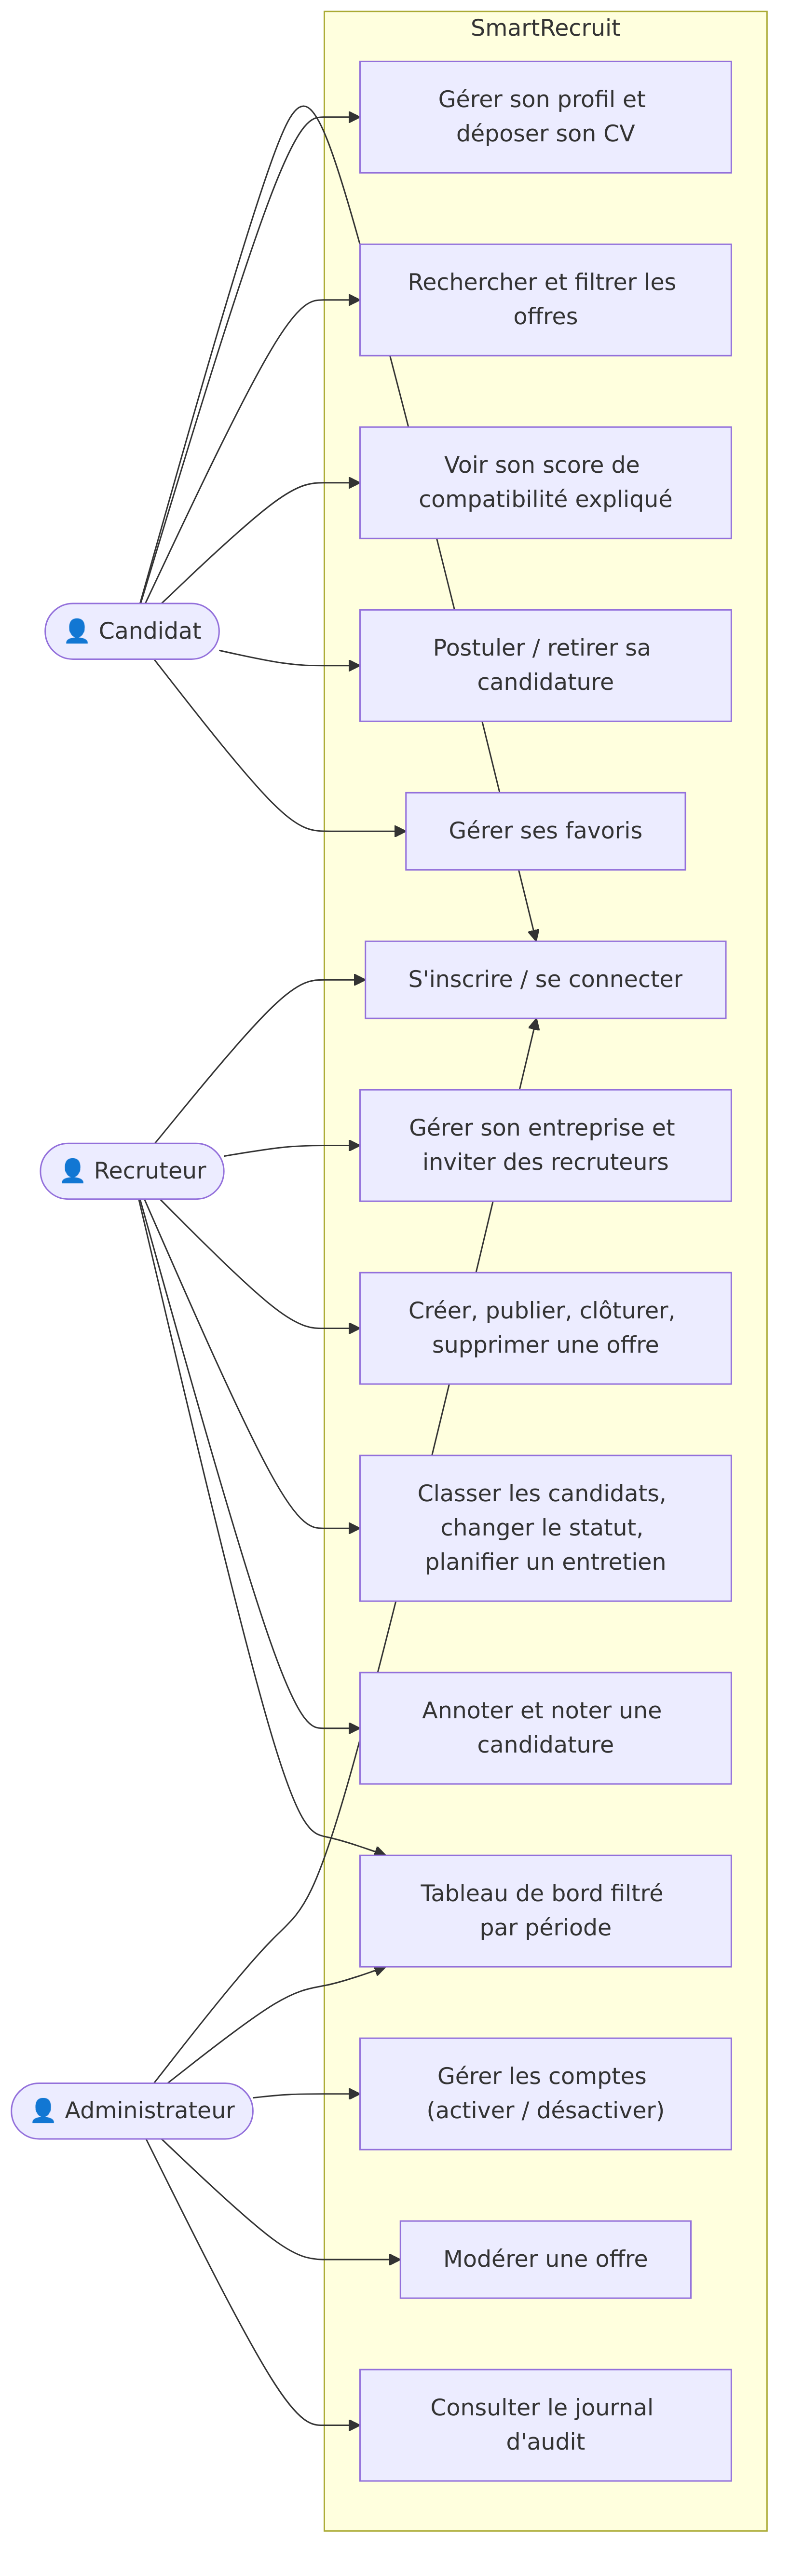
\includegraphics[keepaspectratio]{../images/diagramme-1.png}}
\caption{Cas d\textquotesingle utilisation par rôle}
\end{figure}

\section{2. Architecture}\label{2-architecture}

\begin{figure}
\centering
\pandocbounded{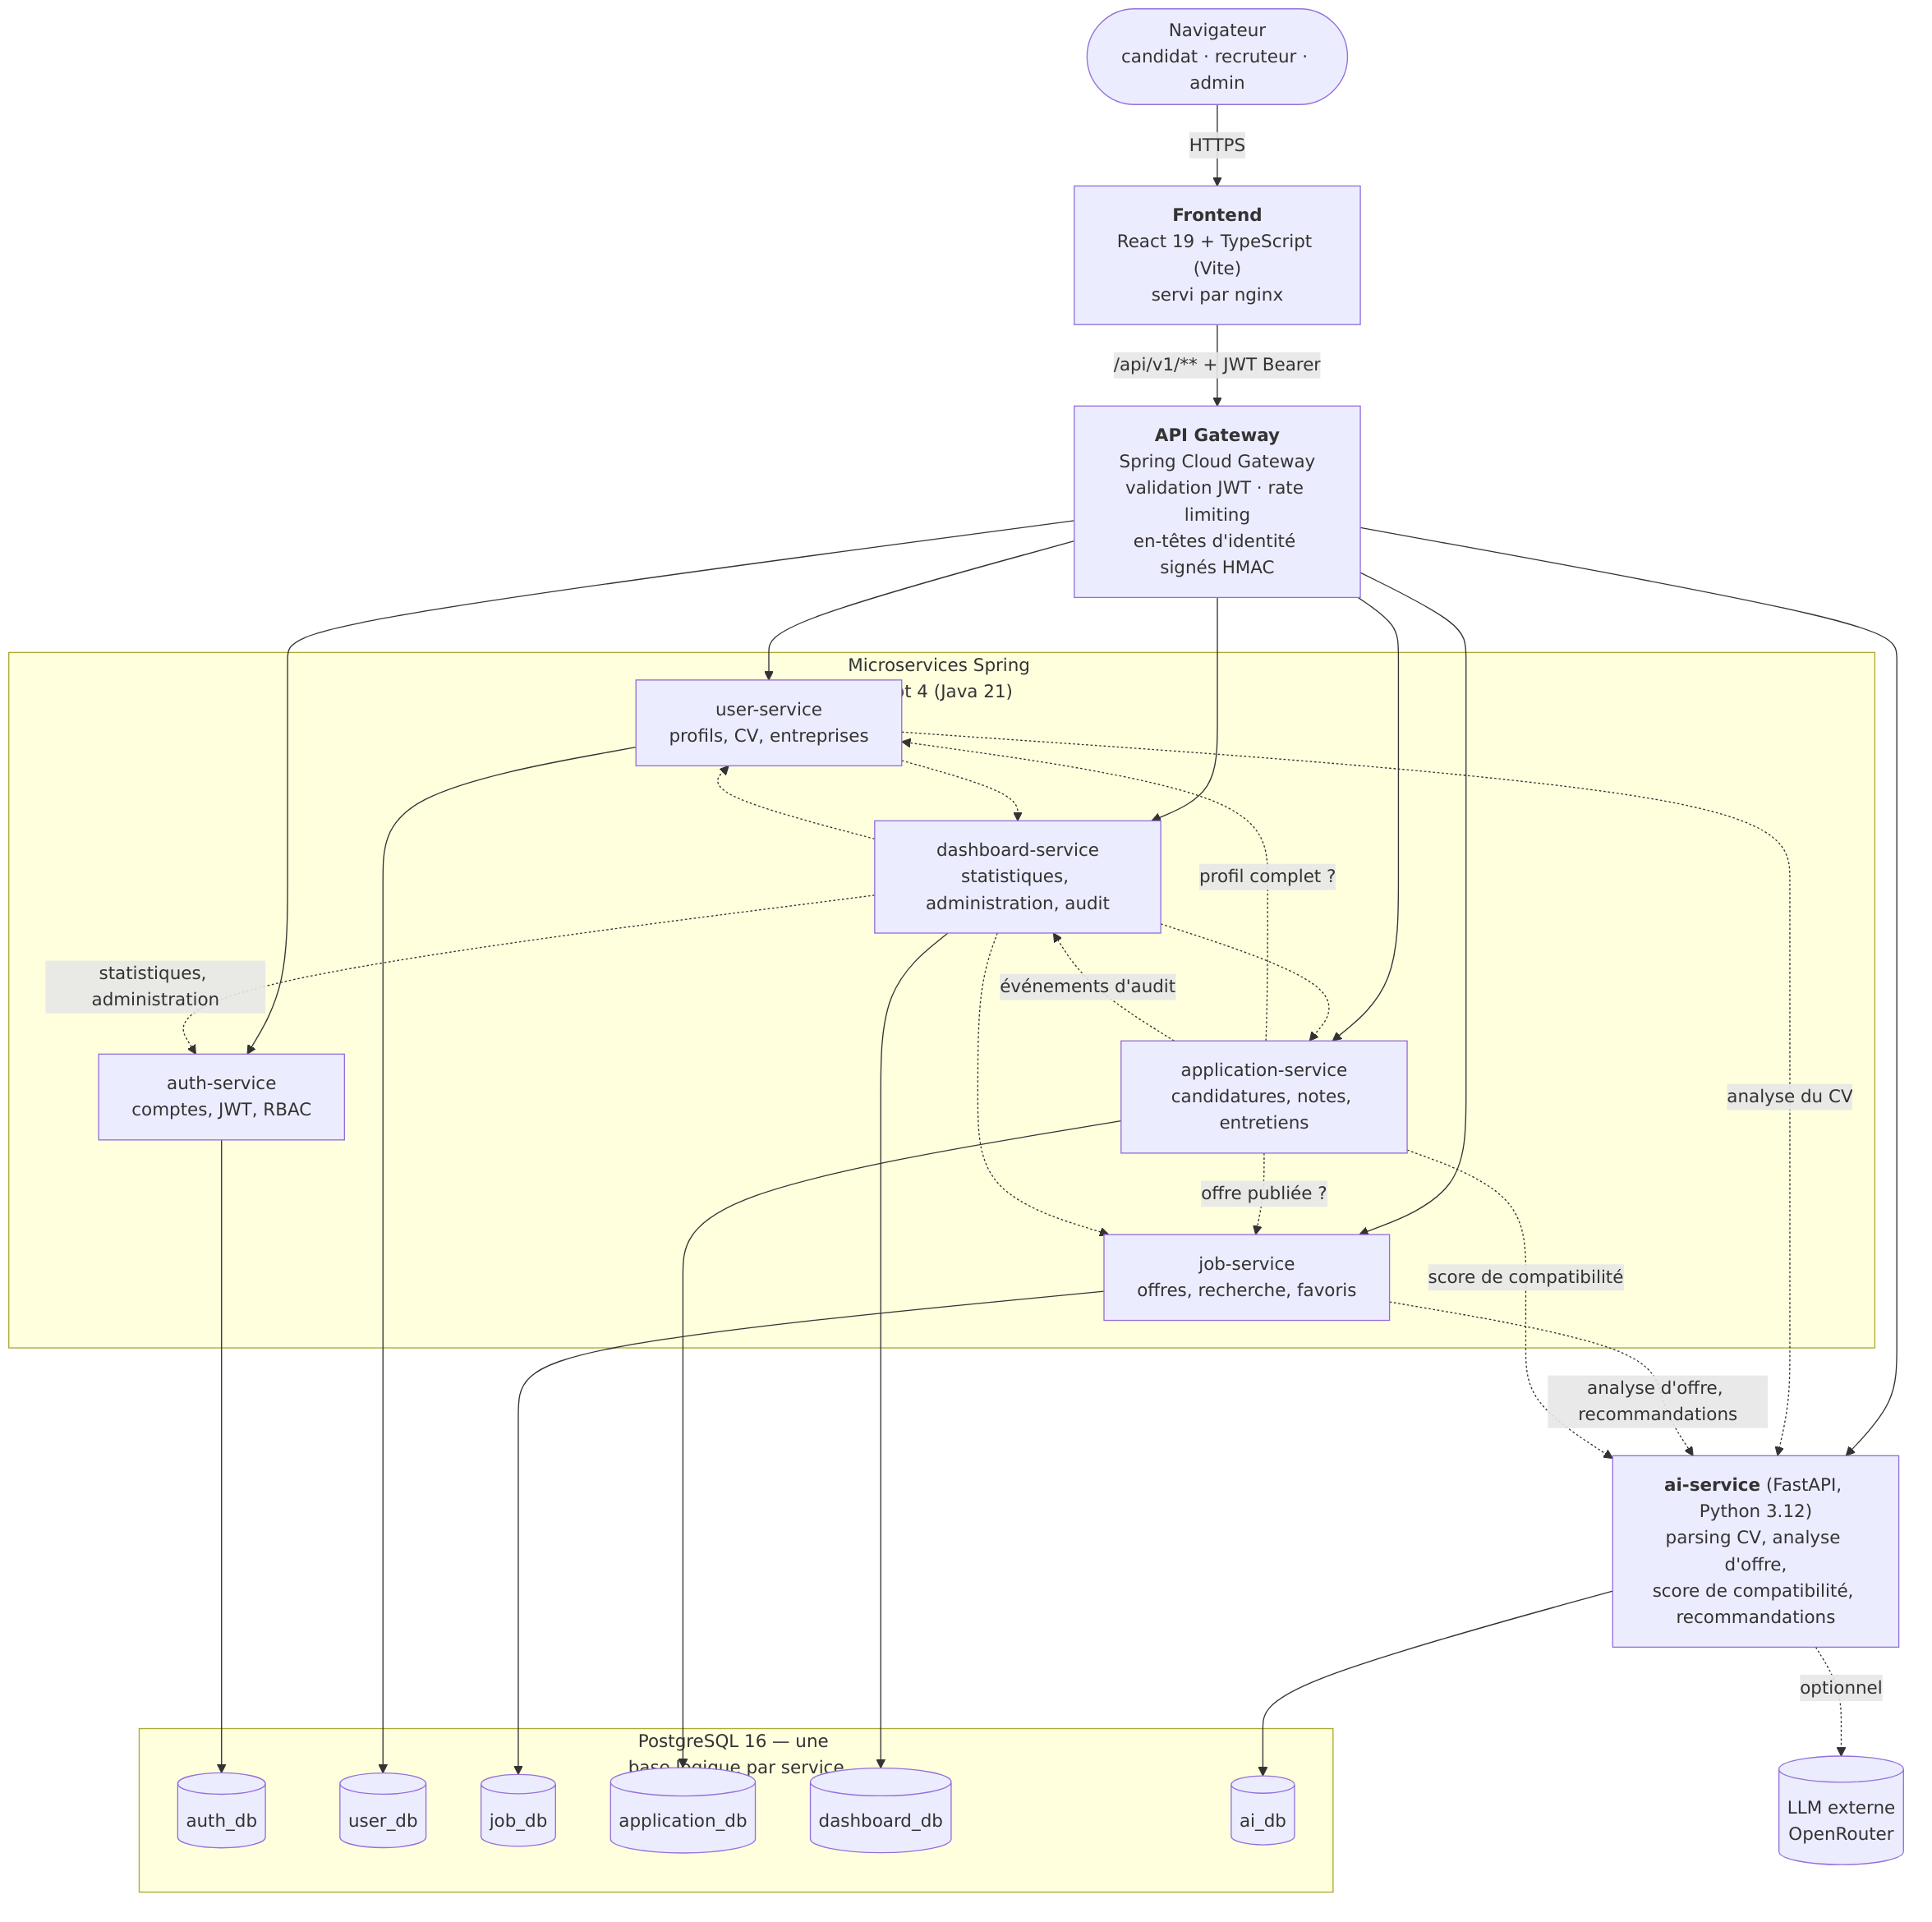
\includegraphics[keepaspectratio]{../images/diagramme-2.png}}
\caption{Architecture : frontend, API Gateway, microservices et bases
PostgreSQL}
\end{figure}

\begin{itemize}
\tightlist
\item
  \textbf{6 microservices Spring Boot 4 (Java 21)} + \textbf{1 service
  IA FastAPI (Python 3.12)} + \textbf{SPA React}.
\item
  \textbf{Architecture en couches dans chaque service} :
  \texttt{controller/}\allowbreak{}\texttt{\ →\ service/}\allowbreak{}\texttt{\ →\ repository/}\allowbreak{}\texttt{\ →\ model/}\allowbreak{},
  plus \texttt{dto/}, \texttt{config/}, \texttt{security/},
  \texttt{exception/}, \texttt{client/} (appels inter-services). Le
  frontend sépare \texttt{api/} (accès HTTP), \texttt{auth/},
  \texttt{components/}, \texttt{pages/}, \texttt{lib/}.
\item
  \textbf{Sécurité par conception} : seul le gateway est exposé côté
  navigateur ; il valide le JWT puis transmet l\textquotesingle identité
  dans des en-têtes signés HMAC-SHA256 que chaque service vérifie (un
  appel direct sans signature est rejeté en 401). Toutes les chaînes
  JSON entrantes sont assainies (jsoup) contre le XSS ; accès aux
  données uniquement par JPA/JPQL paramétré (pas
  d\textquotesingle injection SQL).
\item
  \textbf{Tolérance aux pannes par conception} : l\textquotesingle IA
  est appelée en « best effort » (une offre ou une candidature reste
  valide si l\textquotesingle IA est indisponible, le score reste
  \texttt{null}) ; l\textquotesingle analyse IA d\textquotesingle une
  offre échouée est relancée automatiquement ; le gateway échoue en
  moins de 3 s si un service est arrêté.
\item
  \textbf{Déploiement} : Docker Compose (local), Kubernetes (Kustomize,
  Helm), Terraform, Ansible, CI/CD GitHub Actions avec déploiement sur
  une VM Azure et tests de fumée. Observabilité : Prometheus/Grafana,
  ELK. Détails : \href{../DEVOPS.pdf}{DEVOPS.md}.
\end{itemize}

\begin{figure}
\centering
\pandocbounded{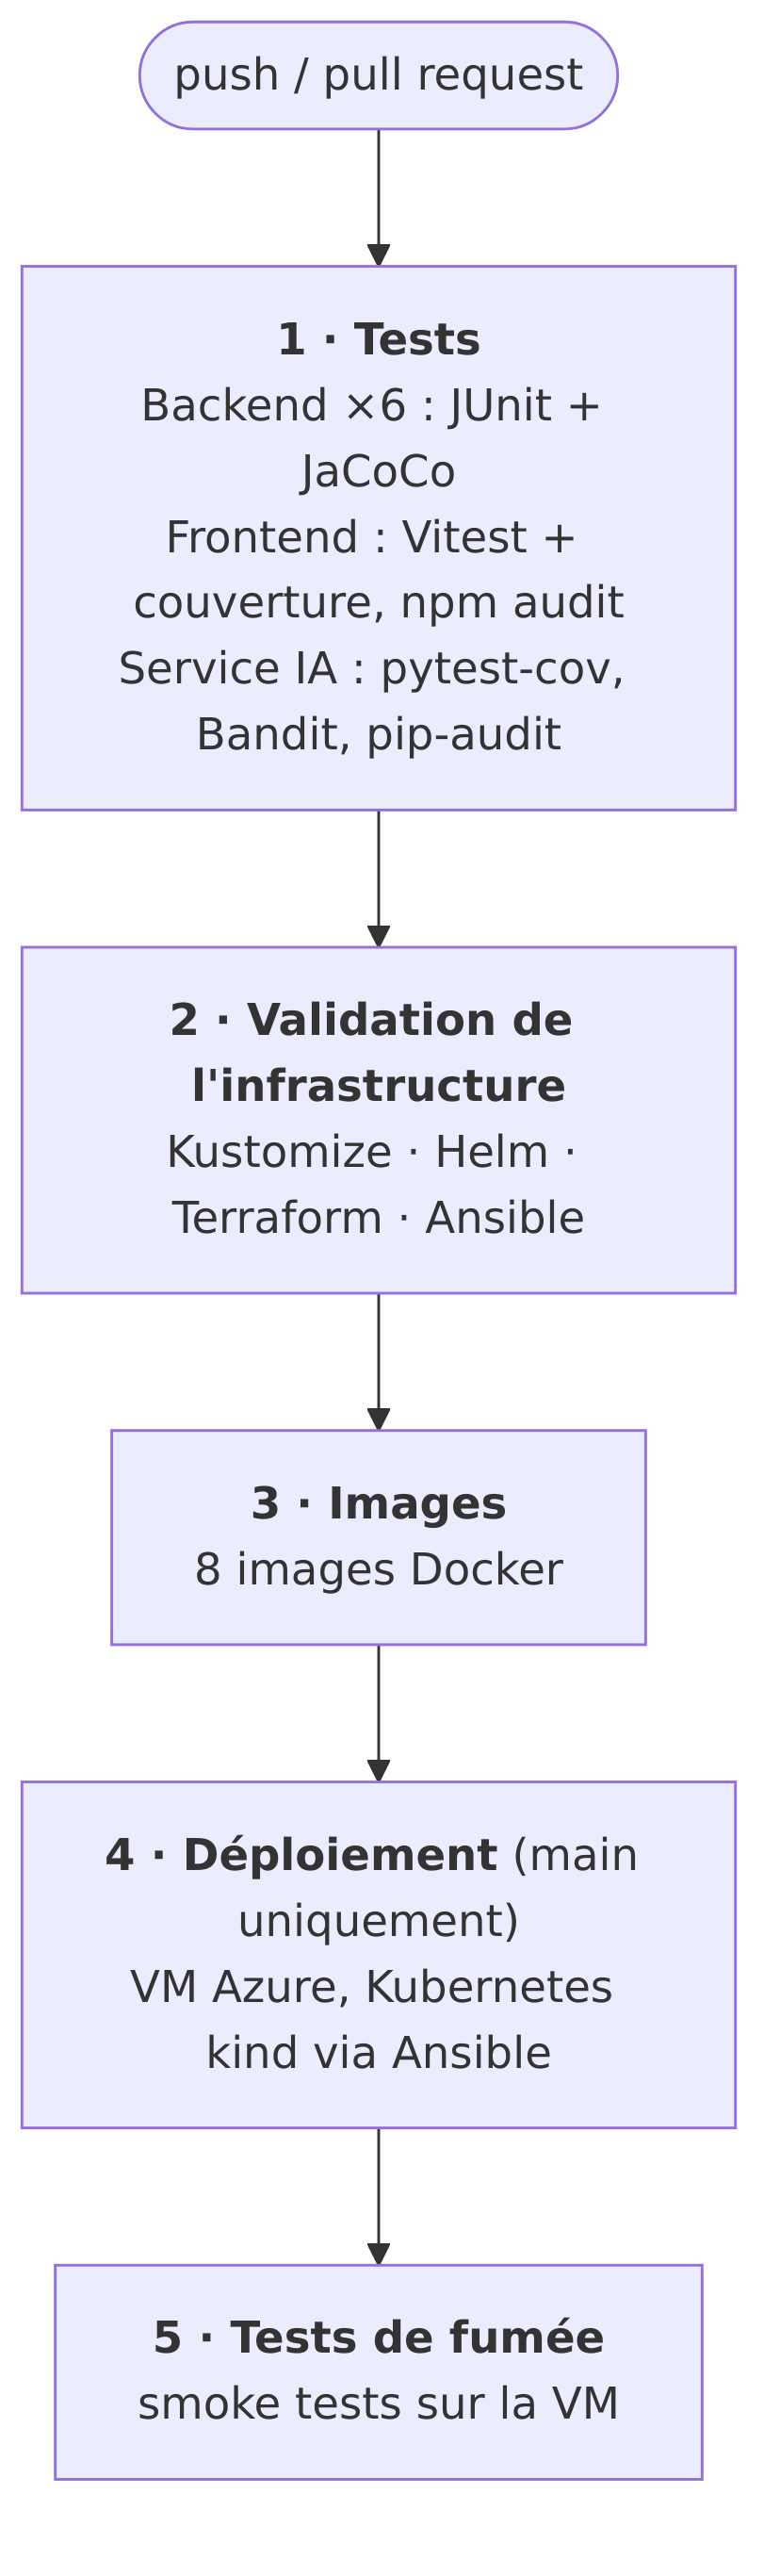
\includegraphics[keepaspectratio]{../images/diagramme-8.png}}
\caption{Pipeline CI/CD (GitHub Actions)}
\end{figure}

\section{3. Modèle de données}\label{3-moduxe8le-de-donnuxe9es}

Référence complète : \href{../DATA_MODEL.pdf}{DATA\_MODEL.md} et
\href{../API_CONTRACTS.pdf}{API\_CONTRACTS.md}.

\begin{figure}
\centering
\pandocbounded{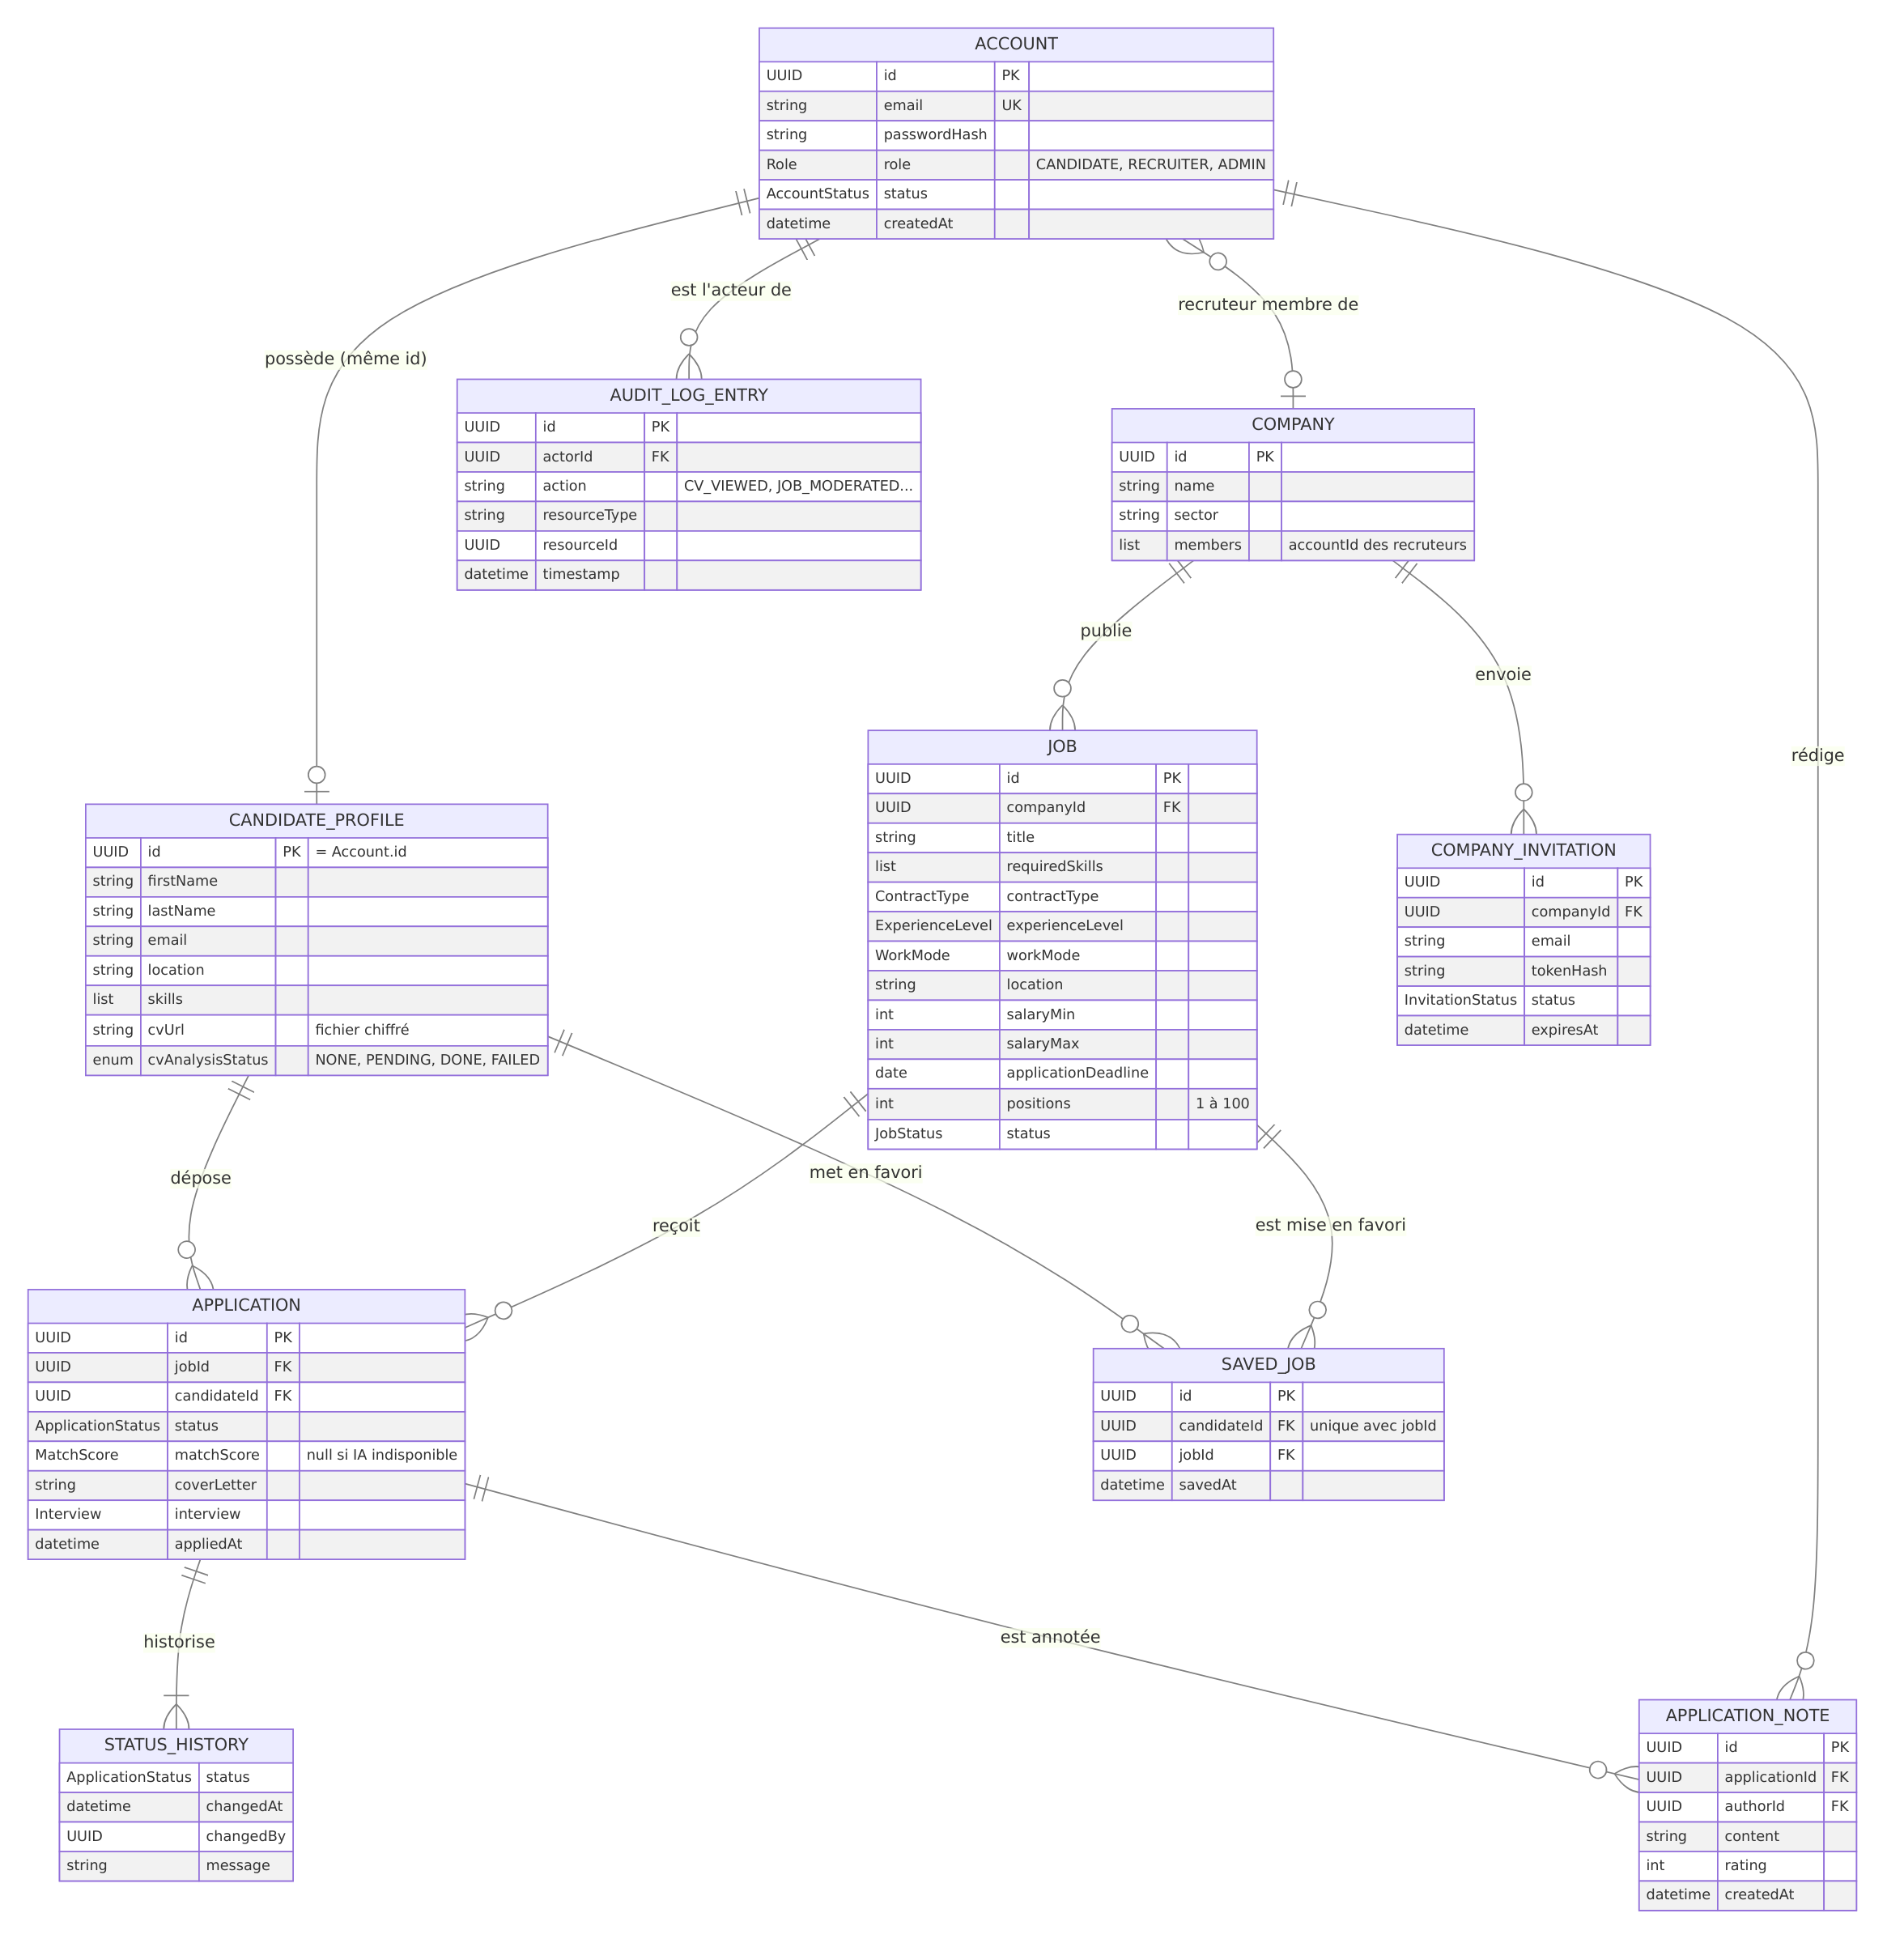
\includegraphics[keepaspectratio]{../images/diagramme-3.png}}
\caption{Modèle de données}
\end{figure}

\begin{longtable}[]{@{}
  >{\raggedright\arraybackslash}p{(\linewidth - 4\tabcolsep) * \real{0.2192}}
  >{\raggedright\arraybackslash}p{(\linewidth - 4\tabcolsep) * \real{0.3836}}
  >{\raggedright\arraybackslash}p{(\linewidth - 4\tabcolsep) * \real{0.3973}}@{}}
\toprule\noalign{}
\begin{minipage}[b]{\linewidth}\raggedright
Relation
\end{minipage} & \begin{minipage}[b]{\linewidth}\raggedright
Cardinalité
\end{minipage} & \begin{minipage}[b]{\linewidth}\raggedright
Mise en œuvre
\end{minipage} \\
\midrule\noalign{}
\endhead
\bottomrule\noalign{}
\endlastfoot
Company --- Job & 1-N & \texttt{Job.companyId} \\
Job --- Application & 1-N & \texttt{Application.jobId} \\
Candidat --- Job & \textbf{N-N} via \texttt{Application} (entité
d\textquotesingle association portant statut, score, historique) &
\texttt{(candidate}\allowbreak{}\texttt{Id,\ job}\allowbreak{}\texttt{Id)} \\
Candidat --- Job (favoris) & \textbf{N-N} via \texttt{SavedJob} & clé
unique
\texttt{(candidate}\allowbreak{}\texttt{Id,\ job}\allowbreak{}\texttt{Id)} \\
Company --- Recruteurs & 1-N & \texttt{Company.members} (un recruteur
n\textquotesingle appartient qu\textquotesingle à une entreprise) \\
Application --- ApplicationNote & 1-N &
\texttt{Application}\allowbreak{}\texttt{Note.}\allowbreak{}\texttt{application}\allowbreak{}\texttt{Id}
(clé étrangère JPA) \\
Account --- CandidateProfile & 1-1 & même identifiant \\
\end{longtable}

Entre microservices, les clés sont des \textbf{clés étrangères logiques}
(chaque service possède sa base) ; la cohérence est garantie par les
appels inter-services (ex. une candidature vérifie que
l\textquotesingle offre existe et est \texttt{PUBLISHED}).

CRUD complet (les 4 opérations) sur 6 entités :

\begin{longtable}[]{@{}
  >{\raggedright\arraybackslash}p{(\linewidth - 8\tabcolsep) * \real{0.1000}}
  >{\raggedright\arraybackslash}p{(\linewidth - 8\tabcolsep) * \real{0.2182}}
  >{\raggedright\arraybackslash}p{(\linewidth - 8\tabcolsep) * \real{0.1818}}
  >{\raggedright\arraybackslash}p{(\linewidth - 8\tabcolsep) * \real{0.2000}}
  >{\raggedright\arraybackslash}p{(\linewidth - 8\tabcolsep) * \real{0.3000}}@{}}
\toprule\noalign{}
\begin{minipage}[b]{\linewidth}\raggedright
Entité
\end{minipage} & \begin{minipage}[b]{\linewidth}\raggedright
Créer
\end{minipage} & \begin{minipage}[b]{\linewidth}\raggedright
Lire
\end{minipage} & \begin{minipage}[b]{\linewidth}\raggedright
Modifier
\end{minipage} & \begin{minipage}[b]{\linewidth}\raggedright
Supprimer
\end{minipage} \\
\midrule\noalign{}
\endhead
\bottomrule\noalign{}
\endlastfoot
Compte & \texttt{POST\ /auth/register} & \texttt{GET\ /auth/me}, liste
admin & (dés)activation admin, réinitialisation du mot de passe &
effacement RGPD avec le profil candidat \\
Profil candidat &
\texttt{PUT\ /}\allowbreak{}\texttt{users/}\allowbreak{}\texttt{candidates/}\allowbreak{}\texttt{me}
(1re fois) &
\texttt{GET\ /}\allowbreak{}\texttt{users/}\allowbreak{}\texttt{candidates/}\allowbreak{}\texttt{me}
& \texttt{PUT} /
\texttt{PATCH\ /}\allowbreak{}\texttt{users/}\allowbreak{}\texttt{candidates/}\allowbreak{}\texttt{me},
dépôt de CV &
\texttt{DELETE\ /}\allowbreak{}\texttt{users/}\allowbreak{}\texttt{candidates/}\allowbreak{}\texttt{me?confirm=true} \\
Offre & \texttt{POST\ /jobs}, duplication & \texttt{GET\ /jobs},
\texttt{GET\ /jobs/\{id\}} & \texttt{PATCH\ /jobs/\{id\}}, statut &
\texttt{DELETE\ /jobs/\{id\}} (brouillon ; une offre publiée se
clôture) \\
Candidature & \texttt{POST\ /applications} &
\texttt{GET\ /}\allowbreak{}\texttt{applications/}\allowbreak{}\texttt{me},
par offre & changement de statut, entretien &
\texttt{DELETE\ /}\allowbreak{}\texttt{applications/}\allowbreak{}\texttt{\{id\}}
(retrait logique \texttt{WITHDRAWN}) \\
Note d\textquotesingle équipe &
\texttt{POST\ /}\allowbreak{}\texttt{applications/}\allowbreak{}\texttt{\{id\}/}\allowbreak{}\texttt{notes}
& \texttt{GET\ …/notes} &
\texttt{PUT\ …/}\allowbreak{}\texttt{notes/}\allowbreak{}\texttt{\{note}\allowbreak{}\texttt{Id\}}
(auteur) &
\texttt{DELETE\ …/}\allowbreak{}\texttt{notes/}\allowbreak{}\texttt{\{note}\allowbreak{}\texttt{Id\}}
(auteur) \\
Favori &
\texttt{PUT\ /}\allowbreak{}\texttt{jobs/}\allowbreak{}\texttt{\{id\}/}\allowbreak{}\texttt{saved}
& \texttt{GET\ /jobs/saved} & --- (aucun attribut modifiable) &
\texttt{DELETE\ /}\allowbreak{}\texttt{jobs/}\allowbreak{}\texttt{\{id\}/}\allowbreak{}\texttt{saved} \\
\end{longtable}

Entreprises : création, lecture, modification, invitations (pas de
suppression : les offres et candidatures en dépendent).

\section{4. Workflows à statuts}\label{4-workflows-uxe0-statuts}

\textbf{Candidature}
(\texttt{Application}\allowbreak{}\texttt{Status.}\allowbreak{}\texttt{ALLOWED\_}\allowbreak{}\texttt{TRANSITIONS})
:

\begin{figure}
\centering
\pandocbounded{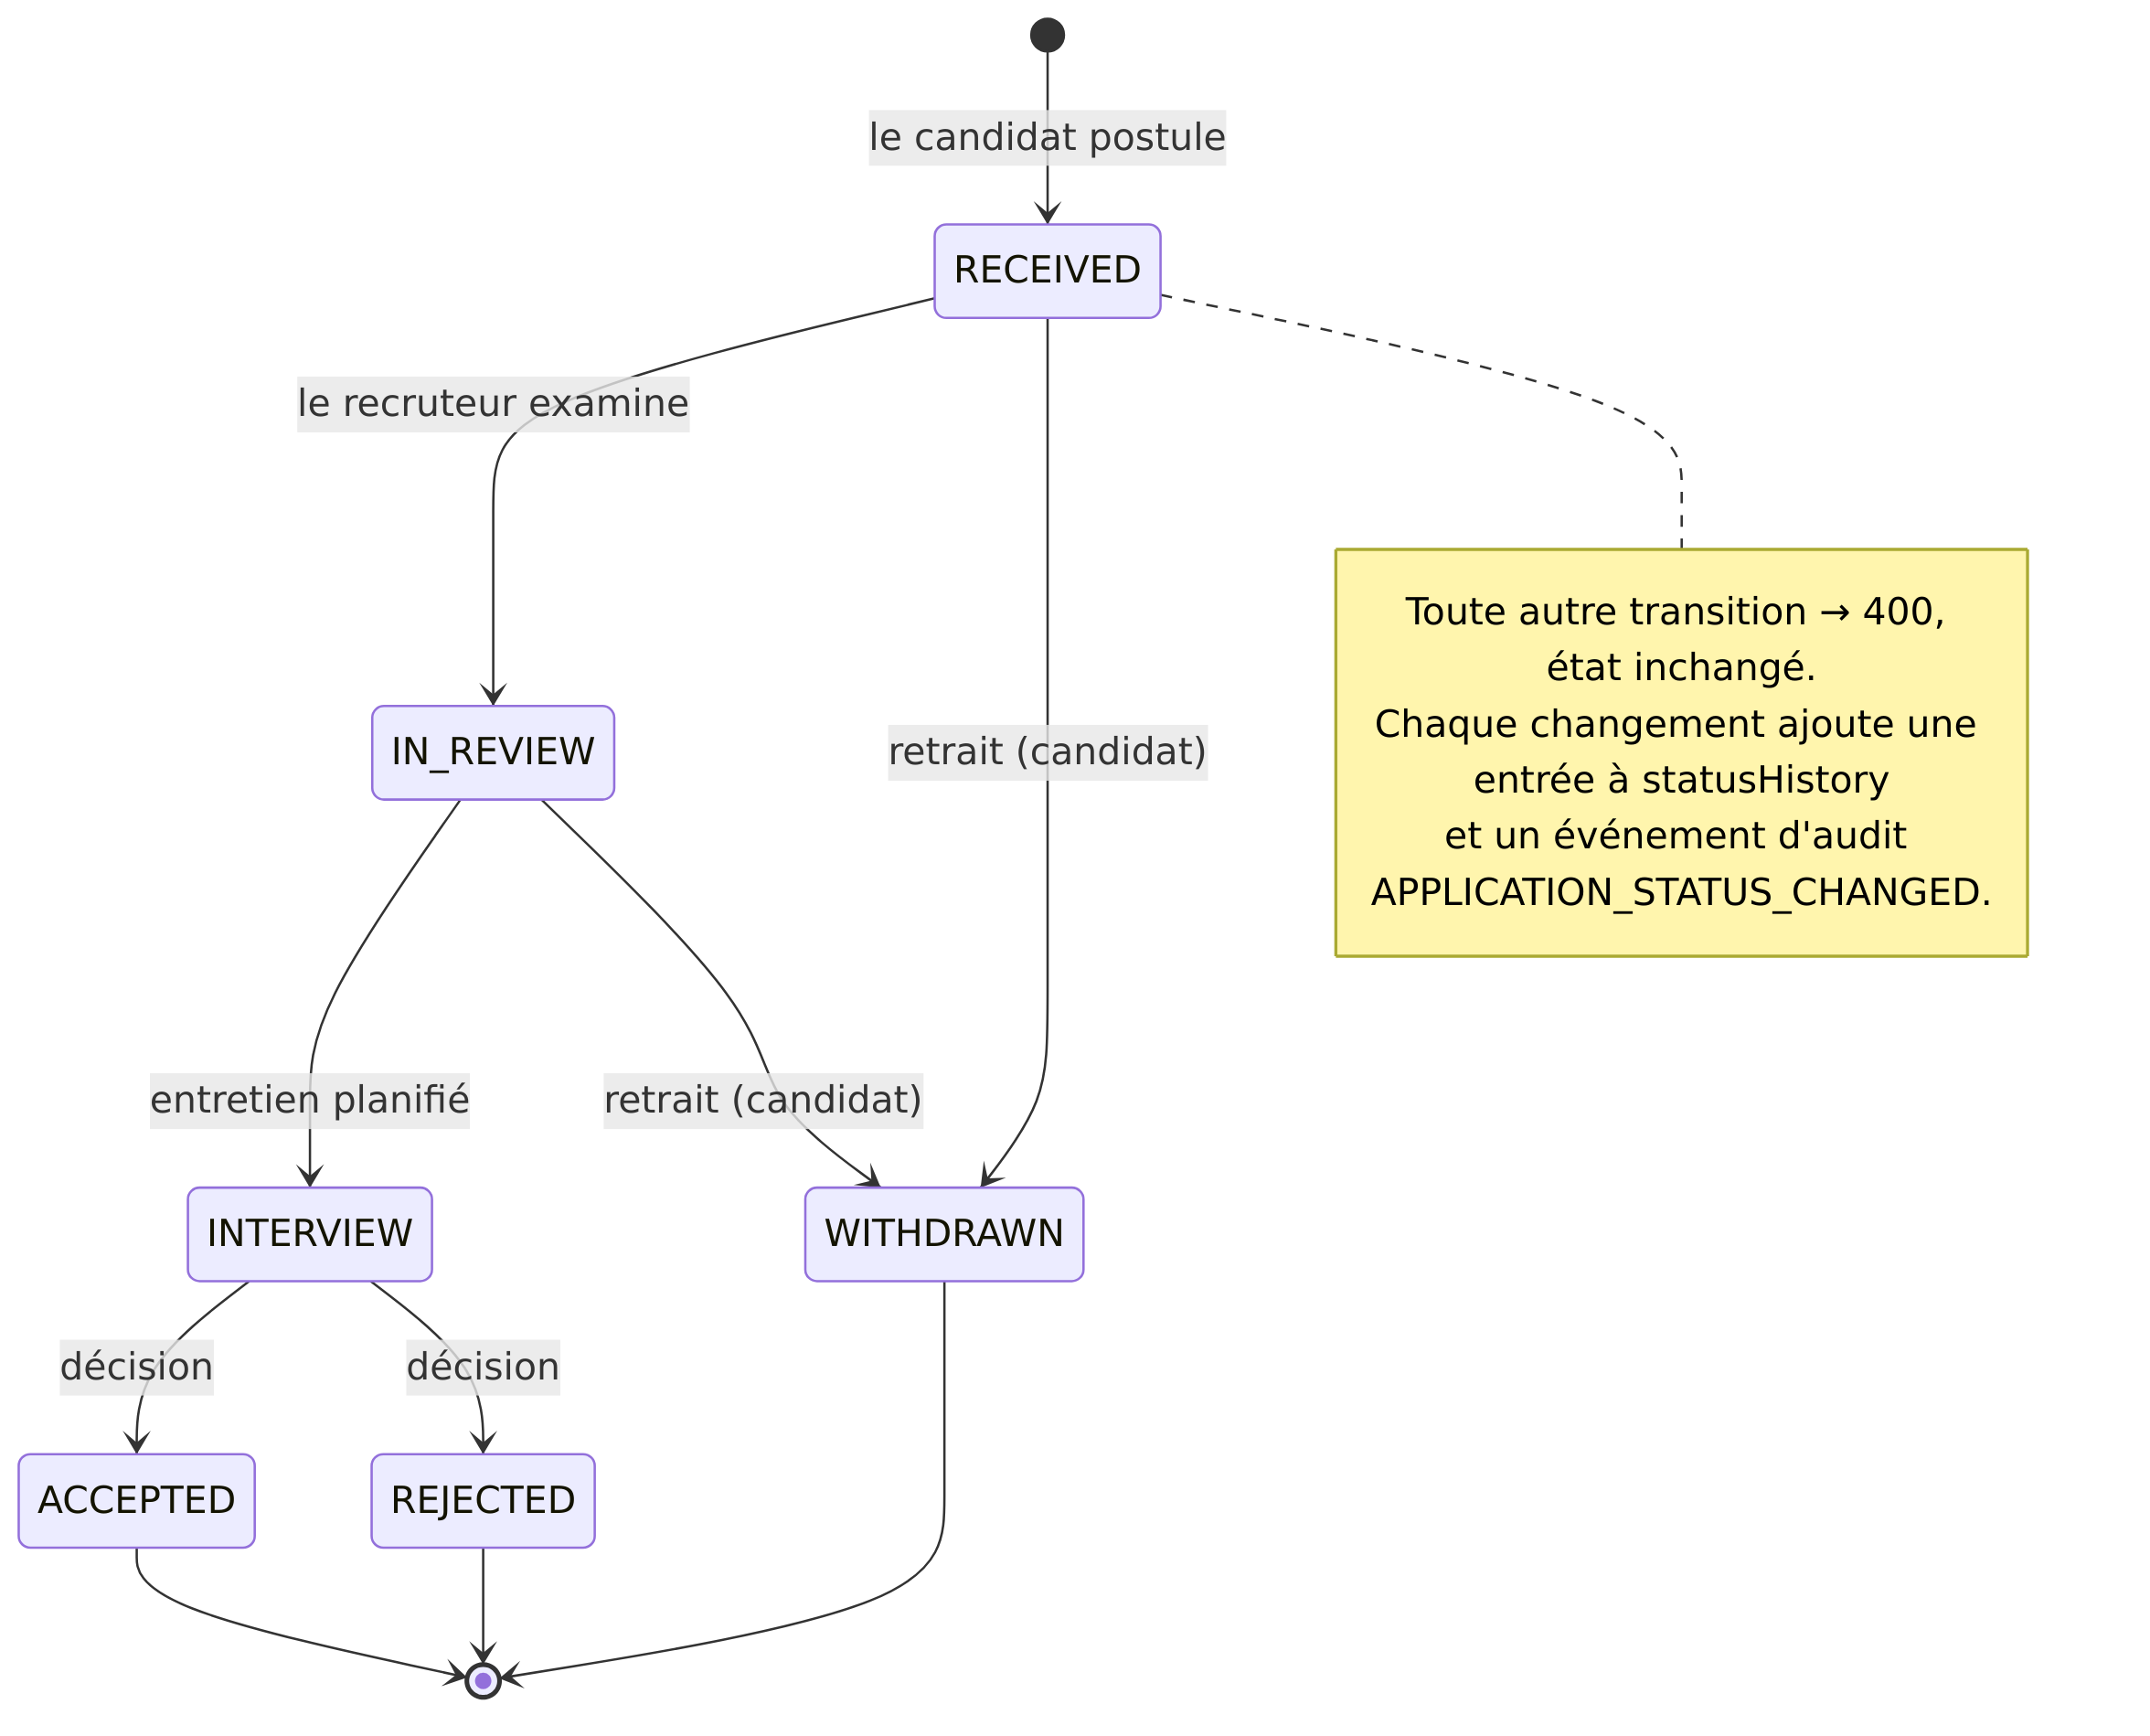
\includegraphics[keepaspectratio]{../images/diagramme-4.png}}
\caption{Workflow d\textquotesingle une candidature (RG‑03)}
\end{figure}

Toute autre transition est rejetée en 400 ; chaque changement ajoute une
entrée à \texttt{statusHistory} et un événement d\textquotesingle audit
\texttt{APPLICATION\_}\allowbreak{}\texttt{STATUS\_}\allowbreak{}\texttt{CHANGED}.

\textbf{Offre} : \texttt{DRAFT\ →\ PUBLISHED},
\texttt{PUBLISHED\ →\ CLOSED}, \texttt{CLOSED\ →\ PUBLISHED} ;
\texttt{MODERATED} (retrait par un admin) bloque toute modification ;
clôture automatique au lendemain de la date limite.

\begin{figure}
\centering
\pandocbounded{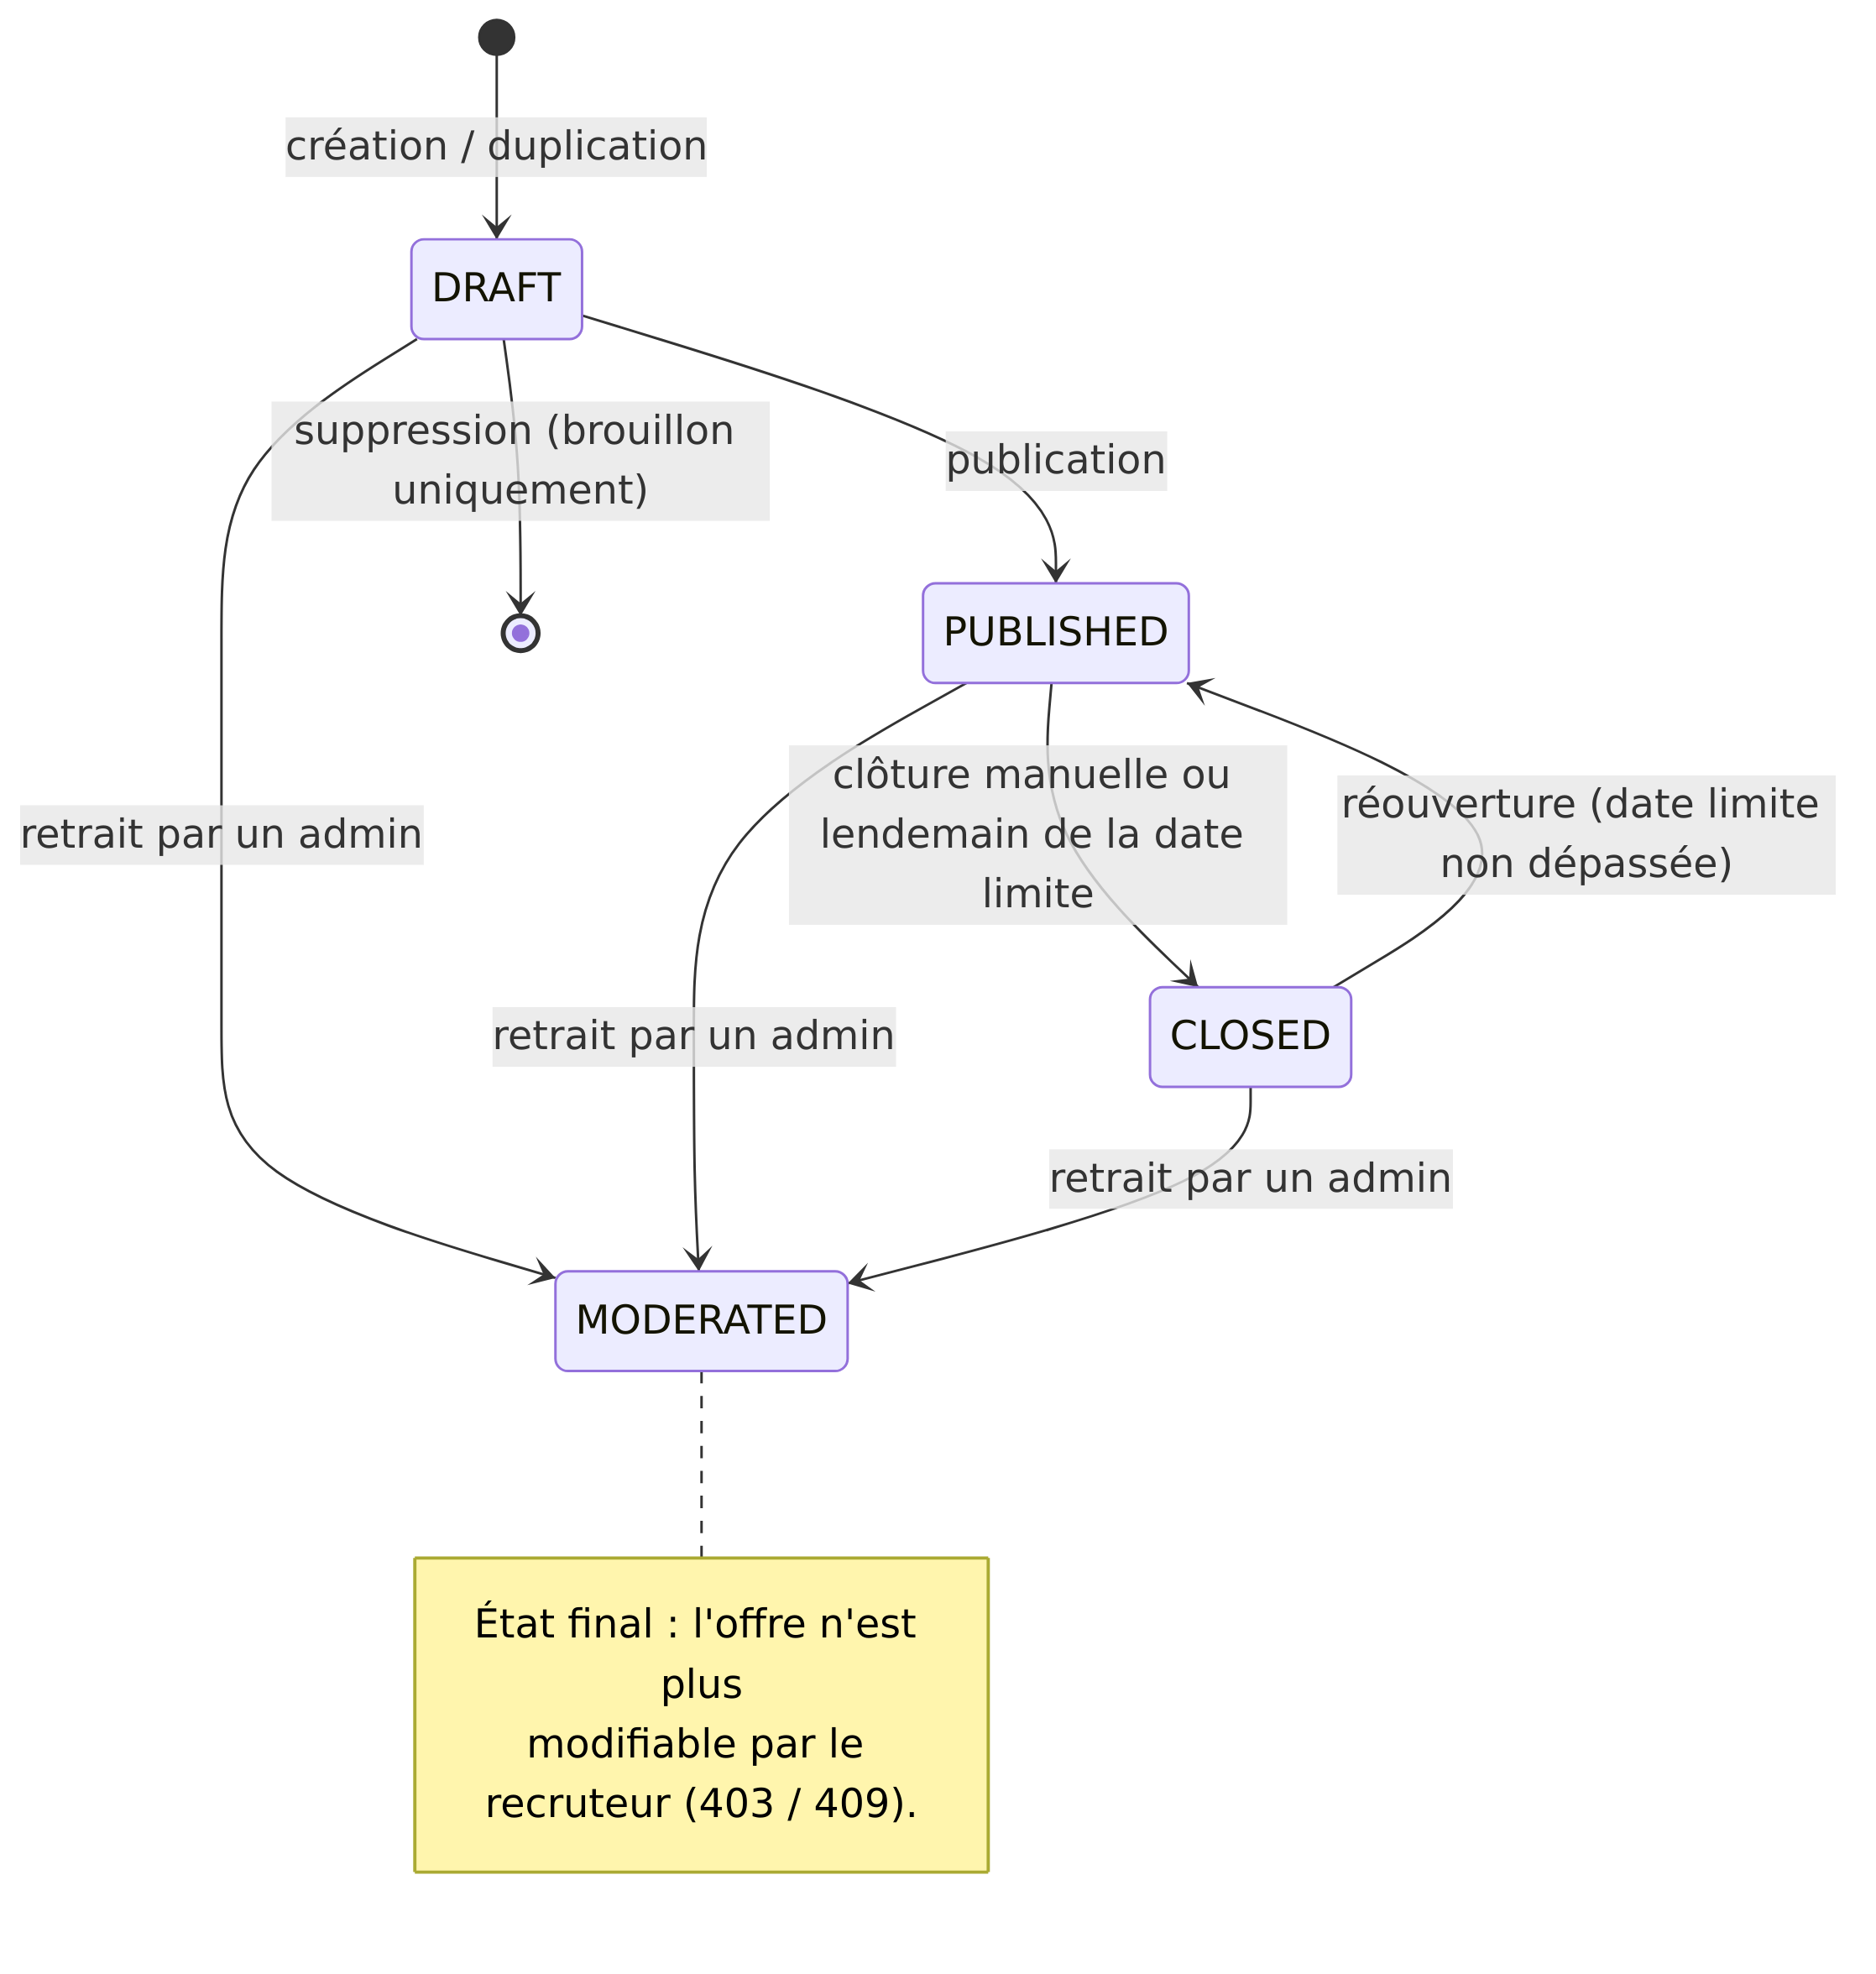
\includegraphics[keepaspectratio]{../images/diagramme-5.png}}
\caption{Workflow d\textquotesingle une offre (RG‑08, RG‑09)}
\end{figure}

\textbf{Postuler à une offre} : le diagramme de séquence ci-après
détaille le parcours de bout en bout (contrôle d\textquotesingle accès,
vérifications RG‑04 et RG‑05, score IA asynchrone en « best effort »).

\begin{figure}
\centering
\pandocbounded{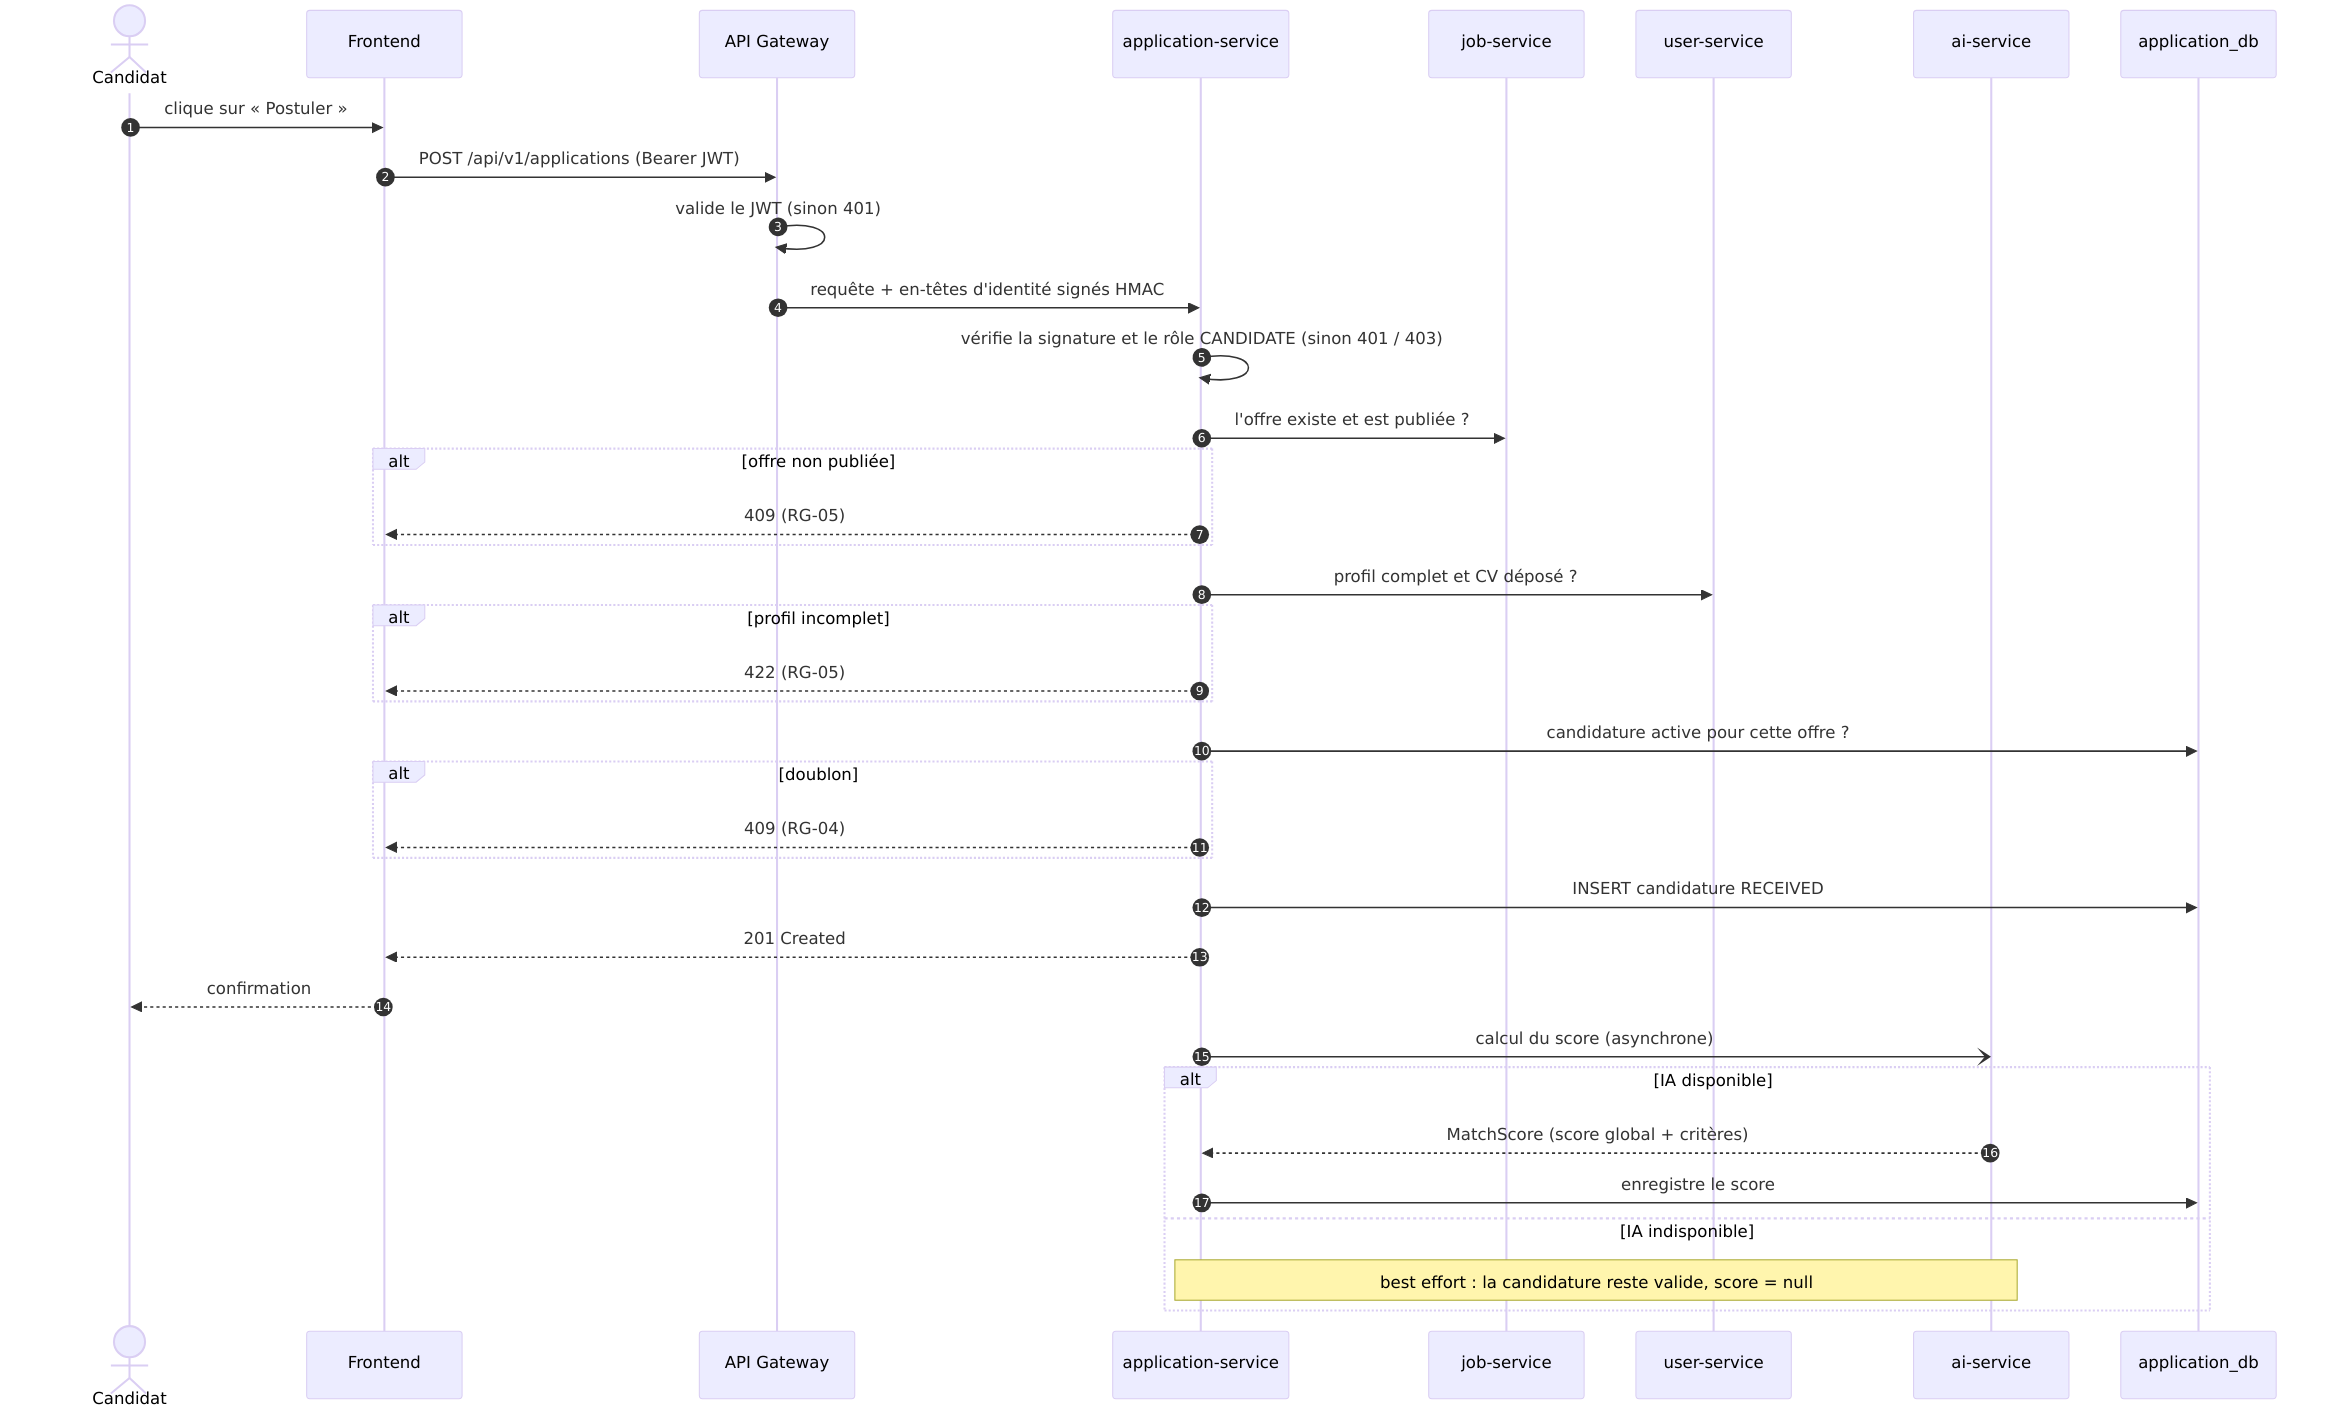
\includegraphics[keepaspectratio]{../images/diagramme-6.png}}
\caption{Séquence : postuler à une offre}
\end{figure}

\section{5. Règles métier explicites et
testables}\label{5-ruxe8gles-muxe9tier-explicites-et-testables}

\begin{longtable}[]{@{}
  >{\raggedright\arraybackslash}p{(\linewidth - 6\tabcolsep) * \real{0.0365}}
  >{\raggedright\arraybackslash}p{(\linewidth - 6\tabcolsep) * \real{0.2044}}
  >{\raggedright\arraybackslash}p{(\linewidth - 6\tabcolsep) * \real{0.2044}}
  >{\raggedright\arraybackslash}p{(\linewidth - 6\tabcolsep) * \real{0.5547}}@{}}
\toprule\noalign{}
\begin{minipage}[b]{\linewidth}\raggedright
Id
\end{minipage} & \begin{minipage}[b]{\linewidth}\raggedright
Règle
\end{minipage} & \begin{minipage}[b]{\linewidth}\raggedright
Comportement attendu
\end{minipage} & \begin{minipage}[b]{\linewidth}\raggedright
Tests
\end{minipage} \\
\midrule\noalign{}
\endhead
\bottomrule\noalign{}
\endlastfoot
RG‑01 & Unicité de l\textquotesingle email d\textquotesingle un compte &
2e inscription avec le même email → 409 &
\texttt{Register}\allowbreak{}\texttt{Integration}\allowbreak{}\texttt{Test.}\allowbreak{}\texttt{register}\allowbreak{}\texttt{With}\allowbreak{}\texttt{Existing}\allowbreak{}\texttt{Email}\allowbreak{}\texttt{Returns409}
; e2e API \\
RG‑02 & Un recruteur n\textquotesingle appartient qu\textquotesingle à
une seule entreprise & 2e création d\textquotesingle entreprise → 409 &
e2e API « seconde entreprise du même recruteur refusée » \\
RG‑03 & Transitions de statut de candidature contrôlées & transitions
hors table → 400, état inchangé &
\texttt{Status}\allowbreak{}\texttt{Change}\allowbreak{}\texttt{Integration}\allowbreak{}\texttt{Test.}\allowbreak{}\texttt{transition}\allowbreak{}\texttt{Table}\allowbreak{}\texttt{Is}\allowbreak{}\texttt{Enforced}
(paramétré) ; fiabilité
\texttt{test\_}\allowbreak{}\texttt{transition\_}\allowbreak{}\texttt{interdite\_}\allowbreak{}\texttt{rejetee\_}\allowbreak{}\texttt{sans\_}\allowbreak{}\texttt{modifier\_}\allowbreak{}\texttt{l\_}\allowbreak{}\texttt{etat} \\
RG‑04 & Une seule candidature active par candidat et par offre & doublon
→ 409 ; possible à nouveau après retrait &
\texttt{Apply}\allowbreak{}\texttt{Integration}\allowbreak{}\texttt{Test.}\allowbreak{}\texttt{can}\allowbreak{}\texttt{Apply}\allowbreak{}\texttt{Again}\allowbreak{}\texttt{After}\allowbreak{}\texttt{Withdrawing},
\texttt{same}\allowbreak{}\texttt{Job}\allowbreak{}\texttt{From}\allowbreak{}\texttt{Another}\allowbreak{}\texttt{Candidate}\allowbreak{}\texttt{Is}\allowbreak{}\texttt{Not}\allowbreak{}\texttt{ADuplicate}
; fiabilité
\texttt{test\_}\allowbreak{}\texttt{double\_}\allowbreak{}\texttt{candidature\_}\allowbreak{}\texttt{rejetee\_}\allowbreak{}\texttt{pas\_}\allowbreak{}\texttt{de\_}\allowbreak{}\texttt{doublon} \\
RG‑05 & Postuler exige une offre publiée, un profil complet et un CV &
offre non publiée → 409 ; profil incomplet → 422 &
\texttt{Apply}\allowbreak{}\texttt{Integration}\allowbreak{}\texttt{Test.}\allowbreak{}\texttt{unpublished}\allowbreak{}\texttt{Job}\allowbreak{}\texttt{Gets409},
\texttt{incomplete}\allowbreak{}\texttt{Profile}\allowbreak{}\texttt{Gets422} \\
RG‑06 & Anti-force brute & 5 échecs en 15 min verrouillent le compte ;
10 requêtes / 5 min / IP sur la connexion et
l\textquotesingle inscription, puis 429 &
\texttt{Login}\allowbreak{}\texttt{Integration}\allowbreak{}\texttt{Test.}\allowbreak{}\texttt{five}\allowbreak{}\texttt{Failures}\allowbreak{}\texttt{Within15}\allowbreak{}\texttt{Minutes}\allowbreak{}\texttt{Lock}\allowbreak{}\texttt{The}\allowbreak{}\texttt{Account}
;
\texttt{Rate}\allowbreak{}\texttt{Limiting}\allowbreak{}\texttt{Integration}\allowbreak{}\texttt{Test}
; preuve d\textquotesingle exécution réelle
\texttt{quality/}\allowbreak{}\texttt{reports/}\allowbreak{}\texttt{security/}\allowbreak{}\texttt{rate-}\allowbreak{}\texttt{limit-}\allowbreak{}\texttt{429.}\allowbreak{}\texttt{txt} \\
RG‑07 & Un administrateur ne peut pas se désactiver lui-même & 400 &
\texttt{Admin}\allowbreak{}\texttt{User}\allowbreak{}\texttt{Integration}\allowbreak{}\texttt{Test.}\allowbreak{}\texttt{an}\allowbreak{}\texttt{Admin}\allowbreak{}\texttt{Cannot}\allowbreak{}\texttt{Disable}\allowbreak{}\texttt{Themself} \\
RG‑08 & Cohérence des offres :
\texttt{salary}\allowbreak{}\texttt{Min\ ≤\ salary}\allowbreak{}\texttt{Max},
1 à 100 postes, clôture automatique après la date limite & 400 ; passage
en \texttt{CLOSED} &
\texttt{Job}\allowbreak{}\texttt{Enrichment}\allowbreak{}\texttt{Integration}\allowbreak{}\texttt{Test.}\allowbreak{}\texttt{patch}\allowbreak{}\texttt{Checks}\allowbreak{}\texttt{The}\allowbreak{}\texttt{Salary}\allowbreak{}\texttt{Range}\allowbreak{}\texttt{Against}\allowbreak{}\texttt{The}\allowbreak{}\texttt{Stored}\allowbreak{}\texttt{Bound},
\texttt{expired}\allowbreak{}\texttt{Offers}\allowbreak{}\texttt{Are}\allowbreak{}\texttt{Closed}\allowbreak{}\texttt{And}\allowbreak{}\texttt{Cannot}\allowbreak{}\texttt{Be}\allowbreak{}\texttt{Reopened} \\
RG‑09 & Workflow des offres ; une offre modérée n\textquotesingle est
plus modifiable & transition interdite → 400 ; offre \texttt{MODERATED}
→ 403/409 &
\texttt{Job}\allowbreak{}\texttt{Status}\allowbreak{}\texttt{Integration}\allowbreak{}\texttt{Test.}\allowbreak{}\texttt{forbidden}\allowbreak{}\texttt{Transitions}\allowbreak{}\texttt{Get400}\allowbreak{}\texttt{And}\allowbreak{}\texttt{Nothing}\allowbreak{}\texttt{Changes},
\texttt{moderated}\allowbreak{}\texttt{Offer}\allowbreak{}\texttt{Is}\allowbreak{}\texttt{Out}\allowbreak{}\texttt{Of}\allowbreak{}\texttt{The}\allowbreak{}\texttt{Recruiters}\allowbreak{}\texttt{Hands}
;
\texttt{Job}\allowbreak{}\texttt{Update}\allowbreak{}\texttt{Integration}\allowbreak{}\texttt{Test.}\allowbreak{}\texttt{closed}\allowbreak{}\texttt{And}\allowbreak{}\texttt{Moderated}\allowbreak{}\texttt{Offers}\allowbreak{}\texttt{Get409} \\
\end{longtable}

\section{6. Choix techniques
justifiés}\label{6-choix-techniques-justifiuxe9s}

\begin{itemize}
\tightlist
\item
  \textbf{Spring Boot (Java 21)} pour le cœur métier : écosystème mature
  pour la sécurité (Spring Security), la persistance (JPA) et les tests
  d\textquotesingle intégration (MockMvc, H2), adapté à une architecture
  en couches et en microservices.
\item
  \textbf{FastAPI (Python)} pour l\textquotesingle IA :
  l\textquotesingle écosystème Python est la référence pour le
  traitement de CV (extraction PDF, règles, appel LLM) ; FastAPI apporte
  la validation par schémas (Pydantic) et une documentation OpenAPI
  automatique.
\item
  \textbf{React + TypeScript} : typage statique partagé avec les
  contrats d\textquotesingle API, tests de composants rapides (Vitest,
  Testing Library) ; \textbf{PostgreSQL} pour
  l\textquotesingle intégrité transactionnelle ; \textbf{Docker Compose
  / Kubernetes} pour une installation reproductible (portabilité).
\end{itemize}

\section{7. Qualité intégrée dès la conception (ISO/IEC
25010)}\label{7-qualituxe9-intuxe9gruxe9e-duxe8s-la-conception-isoiec-25010}

\begin{longtable}[]{@{}
  >{\raggedright\arraybackslash}p{(\linewidth - 2\tabcolsep) * \real{0.3488}}
  >{\raggedright\arraybackslash}p{(\linewidth - 2\tabcolsep) * \real{0.6512}}@{}}
\toprule\noalign{}
\begin{minipage}[b]{\linewidth}\raggedright
Caractéristique
\end{minipage} & \begin{minipage}[b]{\linewidth}\raggedright
Décision de conception
\end{minipage} \\
\midrule\noalign{}
\endhead
\bottomrule\noalign{}
\endlastfoot
Aptitude fonctionnelle & Contrats d\textquotesingle API écrits avant le
code (\texttt{API\_CONTRACTS.md}), enums partagés à
l\textquotesingle identique entre les 3 composants \\
Efficacité de performance & Pagination systématique
(\texttt{size\ ≤\ 50}), cache des scores IA \texttt{(candidat,\ offre)},
appels IA asynchrones \\
Compatibilité & SPA standard (pas d\textquotesingle API propriétaire
navigateur), API REST/JSON, service IA interchangeable (règles ou LLM
externe OpenRouter) \\
Facilité d\textquotesingle utilisation & Libellés visibles sur tous les
champs, messages d\textquotesingle erreur explicites, lien
d\textquotesingle évitement, navigation clavier, mise en page mobile \\
Fiabilité & IA « best effort », relance automatique des analyses, délai
de connexion borné au gateway, transactions JPA \\
Sécurité & JWT + RBAC, en-têtes internes signés, assainissement XSS,
requêtes paramétrées, rate limiting, CV chiffrés, effacement RGPD \\
Maintenabilité & Couches strictes, un service par domaine, tests à
chaque couche, lint (ruff, oxlint) en CI \\
Portabilité & Images Docker pour chaque composant, configuration par
variables d\textquotesingle environnement, manifestes Kubernetes/Helm \\
\end{longtable}

\begin{figure}
\centering
\pandocbounded{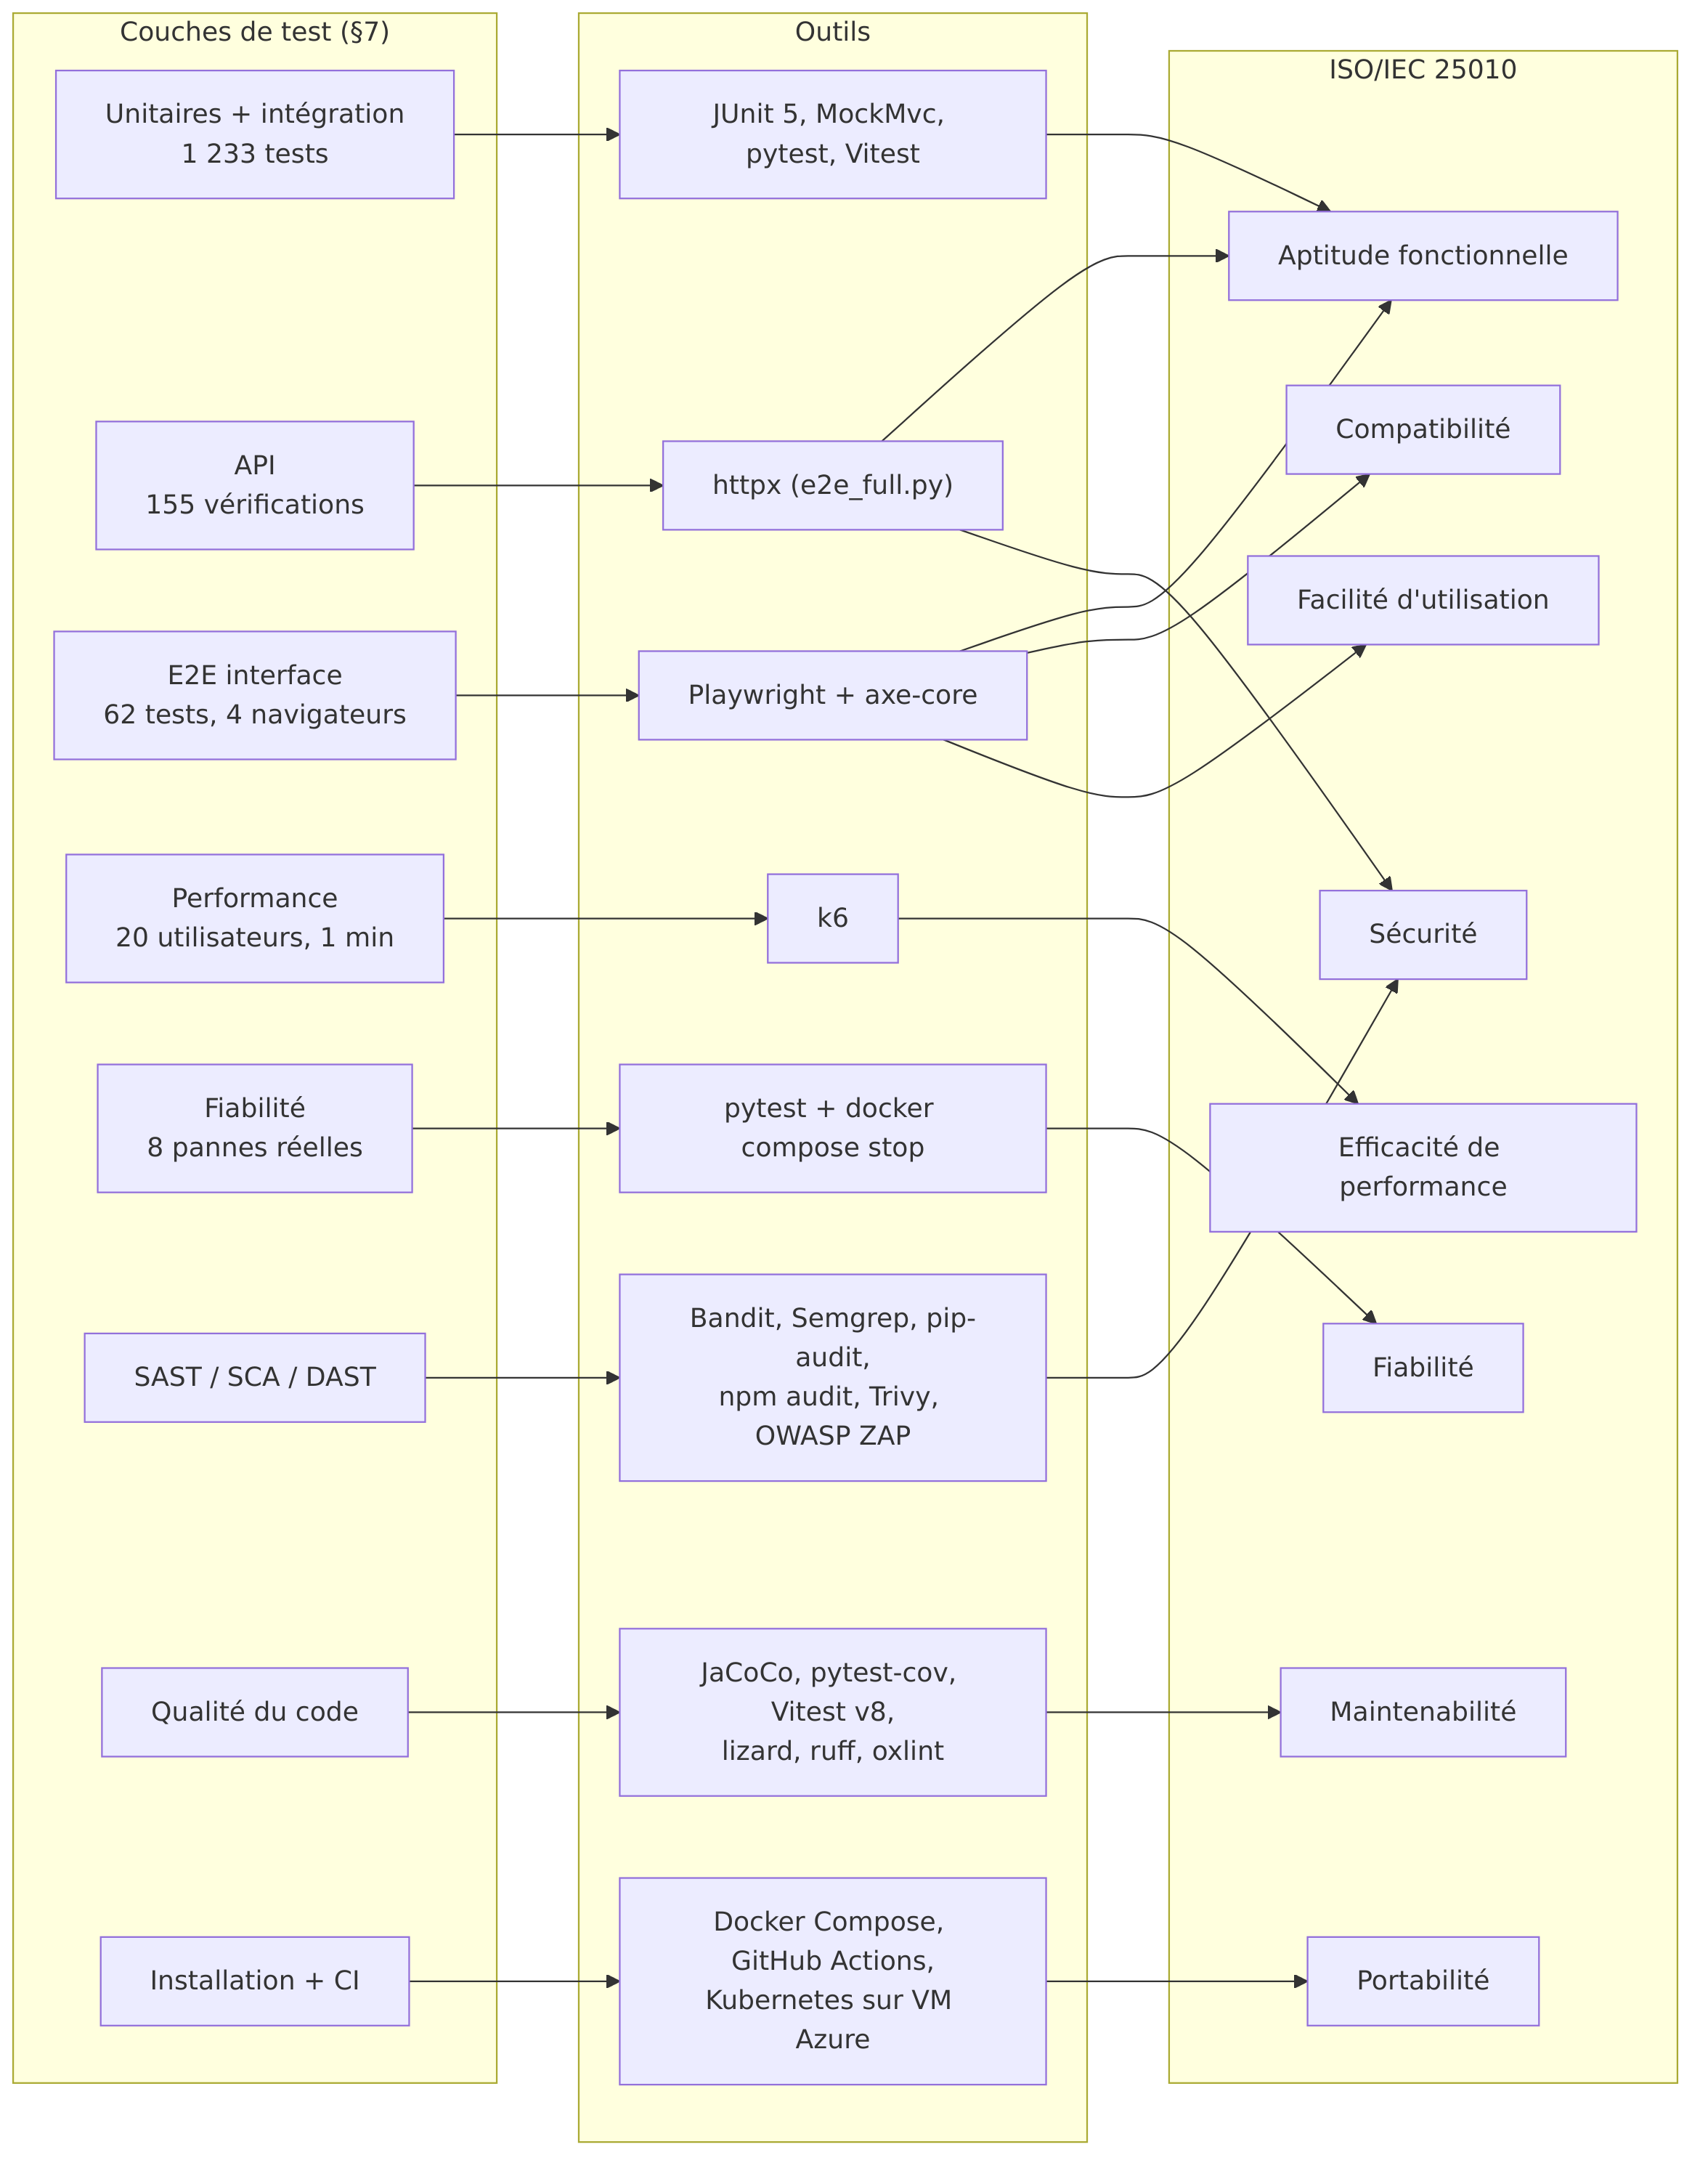
\includegraphics[keepaspectratio]{../images/diagramme-7.png}}
\caption{Stratégie de test : couches → outils → caractéristiques ISO/IEC
25010}
\end{figure}

\end{document}
